\setchapterstyle{kao}
\setchapterpreamble[u]{\margintoc}
\chapter[Environmental sensing with voltage, current and resistance]{Introduction to circuits: Environmental sensing with voltage, current and resistance}
\labch{circuits_intro}
Natural environments and the ecosystems within them are governed by physical characteristics like temperature, light intensity, $O_2$ concentration, $pH$, seawater salinity, and wind or current velocity.
Instruments for environmental sensing generate electrical signals that vary with one or more of these characteristics.
For this to be useful, the relationship between electrical outputs and environmental inputs must be consistent and quantifiable.
The process of establishing this quantitative relationship is called \emph{calibration}.
A calibration usually must work in both directions:
First, the calibration is established by measuring the electrical signals across a relevant range of known environmental conditions.
Then,  electrical signals are acquired from unknown environmental samples, and the calibration is used to infer the conditions under which they were obtained.
This chapter will guide you through the methods and process of designing and building devices to measure electrical signals, and calibrating those devices to quantify environmental conditions.

Because most environmental characteristics vary continuously, the electrical signals generated by environmental sensors are also usually continuous.
These signals are referred to as \emph{analog} signals, to distinguish them from \emph{digital} signals like those you worked with in \refch{first_exercises}.
Digital signals are simply ``high'' or ``low'' --- usually determined by a voltage that is above or below a threshold voltage.
Because analog signals vary continuously, they potentially carry much more information.
However, analog signals must typically be measured much more accurately and precisely than digital signals.
For this reason, analog measurements are handled differently by microcontrollers, with distinct methods and constraints.

Most microcontrollers can directly measure just two parameters: voltage and time.
Unsurprisingly, the vast majority of analog sensors provide information using one or both of these parameters.
A voltage-based analog sensor typically has three connections: ground, \texttt{GND} (\texttt{0V}); an input voltage, $V_{in}$; and, a data output voltage, $V_{data}$.
The data output voltage, $V_{data}$, represents environmental characteristics in the form of a voltage that varies between \texttt{GND} and $V_{in}$.
For example, in \refsec{cal_therm}, you will measure temperature with a component called a thermistor.
A thermistor has a \emph{resistance} (impediment to the flow of electrons) that changes as a function of temperature.
You will combine the thermistor with another resistor in a way that causes the output voltage $V_{data}$ to change with temperature.
You will then use a microcontroller to measure $V_{data}$, calculate thermistor resistance, and use a calibration to infer the temperature.

A time-based sensor uses the duration of or interval between events as the key measurement.
For example, in \refsec{cal_sonar}, you will use an acoustic sensor to measure distance to a object.
In this case, the length of time between an initial event --- sending out a pulse of sound --- and a secondary event --- the echo of that pulse arriving back at the source --- indicates the round trip travel time for sound waves.
Calibrated by a knowledge of the speed of sound, this travel time indicates distance.

The following sections explain some electrical principles that you need to understand when working with voltage-based environmental sensors. You will apply that knowledge to measure battery voltage (an important parameter in a field-deployed device!) and thermistor temperature. You will then use time-based sensors to measure distance and light, and combine both time and voltage to measure wind or current velocity.
%\todo{Textbox explaining font conventions for code, units and electrical quantities.}

%like the \texttt{3V3} pin in your \refch{first_exercises} circuits),
%The data connection takes on a voltage anywhere between
%
%have a is the process of generating
%
%calibration must be bidirectional
%
%In this chapter, we explore the relationships between characteristics of the environment --- \etc ---

\section{Measuring voltage}
\labsec{meas_volt}
Voltage is measured on a microcontroller using an \texttt{Analog to Digital Conversion} (\adc) pin.
\adc pins act as inputs, just as digital \texttt{GPIO} pins do in their input modes.
However, reading the value of a digital \texttt{GPIO} pin results in either 1 or 0 (``high'' or ``low'').
In contrast, an \adc pin returns an integer, often referred to as a \emph{count}, that can span a range, e.g. between 0 and 1023 for an 8-bit ADC (as on an ESP8266) or between 0 and 8191 for a 13-bit ADC (as on an ESP32-S2).
The count's value is proportional to the voltage applied to the \adc pin.

For example, in \htmladdnormallink{\texttt{Analog to Digital Conversion} on the ESP8266}{http://docs.micropython.org/en/v1.9.3/esp8266/esp8266/quickref.html\#adc-analog-to-digital-conversion}, an \adc value of 0 implies \texttt{0V}, \adc value of 1023 implies \texttt{1V}, and \adc value of 113 implies $\frac{113}{1024} \times 1\mathtt{V}$ or \texttt{0.11V}.
In general,
\begin{equation}\label{adc_volt}
V = V_{max}\frac{C_{ADC}}{C_{max}+1}
%V \mathsf{V} \mathrm{V} = \frac{ADC}{1024} \frac{\mathsf{ADC}}{1024} \frac{\mathrm{ADC}}{1024}
\end{equation}
 where $C_{ADC}$ is the integer value read from the \adc pin, $V$ is the applied voltage in units of \texttt{volts}, $V_{max}$ is the maximum voltage  that the \adc can sense, and ${C_{max}}$ is the maximum count of the \adc
\sidenote[][*-8]{
	\begin{kaobox}[backgroundcolor=\SNcolor,frametitlebackgroundcolor=\SNcolor,frametitle=Resolve to change!]
		An important implication of Equation \ref{adc_volt} is a limit to the \htmladdnormallink{\emph{resolution}}{https://www.itl.nist.gov/div898/handbook/mpc/section4/mpc451.htm} of the \texttt{ESP8266}'s \adc.
		Resolution is the smallest increment of a physical characteristic that can be distinguished by a sensor.
		In this case, an increment of 1 in the integer value of the \texttt{ESP8266}'s \adc corresponds to a change of voltage, $\Delta V$, of
		\begin{equation}\label{adc_volt2}
		\Delta V = \frac{1~ \mathtt{volts}}{1024} = 0.000977~ \mathtt{volts}
		\end{equation}
		This means that, even if there were no measurement errors associated with accuracy and precision, the \adc reading could represent any voltage within a range of approximately $\pm \frac{1}{2}\Delta V$.
	\end{kaobox}
}.

\subsection{Voltage of an \texttt{18650} lithium-ion battery}
The task at hand in this section is to measure the voltage of a rechargeable lithium-ion battery called an \htmladdnormallink{``\texttt{18650}''}{https://en.wikipedia.org/wiki/Lithium-ion_battery}.
The name \texttt{18650} derives from its dimensions: an \texttt{18650} battery is \texttt{18mm} in diameter and \texttt{65mm} long.
\texttt{18650}s are a common standard of rechargeable battery, widely available and well suited to powering environmental sensors.

\texttt{18650} voltages typically range from 3.7-4.2V, depending on how charged they are, ambient temperature, \etc
For an instrument in the field, the capacity to monitor its own battery level can be valuable.
For example, an instrument on the verge of power failure can, if connected to the Internet, send a message indicating it needs maintenance.
Alternatively, it can be programmed to alter its sampling schedule to stretch whatever power remains over a longer duration, even if less frequently.

Monitoring battery voltage with an \adc that measures voltage seems like an easy task, right?

Well, it \emph{is} pretty easy.
But, there's a wrinkle we need to contend with: \adcs have strict limits to how large a voltage they can tolerate.
In fact, for many types of microcontroller these limits are quite low.
For \texttt{ESP8266}s, the limit is \texttt{1V}, and for \texttt{ESP32} and \texttt{ESP32-S2} chips, the default limit is even lower--as low as \texttt{0.75V} for the \texttt{ESP32-S2}.  However, thankfully, for the \texttt{ESP32} chips, this can be reconfigured in software to as much as approximately \texttt{2.5V}.
In any case, that's much lower than even a mostly discharged \texttt{18650} battery's voltage.
If we attach the terminals of an \texttt{18650} directly to an \texttt{ESP}'s \adc, we risk the destruction of the \adc and possibly other components as well.

We need a way to \emph{represent} the voltage of an \texttt{18650} with a voltage that we know will never exceed the maximum allowable voltage for the \adc.
To accomplish this, we'll create a sensor in the typical 3-connection analog format: \texttt{GND}, $V_{in}$ and $V_{data}$.
In this sensor, \texttt{GND} and $V_{in}$ will come from the \texttt{18650} terminals.
$V_{data}$ will come from the circuit we're about to design, in such a way as to insure that it accurately represents battery voltage according to a known calibration while staying within the limit.

\subsubsection{Ohm's Law for voltage, current and resistance}
The design of our current sensor is based on one of the fundamental laws governing electricity, \htmladdnormallink{Ohm's Law}{https://en.wikipedia.org/wiki/Ohm\%27s\_law}.
Ohm's Law defines the quantitative relationship between voltage, current and resistance across a \htmladdnormallink{\emph{resistor}}{https://en.wikipedia.org/wiki/Resistor}.
You used a resistor when you constructed a circuit to power an external LED in \refsec{ext_led}.
Though we did not go into the details there, the purpose of that resistor was to regulate the amount of current flowing through the LED.
How did we know which resistor to use?
We calculated it using Ohm's Law.

In a diagram of an electrical circuit, a resistor is illustrated by a zig-zag line:
\begin{figure}[h!]
		\labfig{res}
		\centering
%	\begin{center}
		\begin{tikzpicture}[american voltages]
		\draw
		(0,0) to [short,l=$V_{1}$, *-] (1,0)
		to [R, l=$R$, i_=$I$] (3,0)
		to [short,l=$V_{2}$, -*] (4,0);
		\end{tikzpicture}
		\caption[Circuit diagram: Resistor]{Circuit diagram of a resistor.}
%	\end{center}
\end{figure}

In this circuit, $R$ is the value of the resistor.
$V_1$ is the voltage imposed on the left wire from the resistor, and $V_2$ is the voltage imposed on the right wire.
The voltage drop across this resistor is $V = V_1 - V_2$.
The current flowing through the resistor is $I$.

According to Ohm's Law,
\begin{equation}\label{OhmsVIR}
V = I R
\end{equation}
In Equation \ref{OhmsVIR}, $V$ is the voltage difference measured across the resistor, in units of \htmladdnormallink{\texttt{volts}}{https://en.wikipedia.org/wiki/Volt}.
$I$ is the current (i.e., the flow of electrons) through the resistor, in units of \htmladdnormallink{\texttt{amperes}}{https://en.wikipedia.org/wiki/Ampere} (usually shortened to ``\texttt{amps}'').
$R$ is the \emph{resistance} of the conductor, in units of \htmladdnormallink{\texttt{ohms}}{https://en.wikipedia.org/wiki/Ampere}.


\begin{kaobox}[frametitle=Signs of things to come \dots]
Current consists of flowing electrons.
This means that whenever we refer to a value like $I$ to indicate current, we need to be clear about which direction of flow we count as positive.
This will become especially important when we work with more complex circuits later on.

In the circuit diagram, the small arrow above $I$ indicates the direction we choose to count current flow as positive.
We can choose either direction, but we must be consistent in using one direction or the other.
For that reason, the direction of positive current flow will always be indicated in the circuit diagrams in this book.

%Because no electrons are created or lost while passing through the resistor, the current is the same at every point in this simple circuit.

The arrow also tells us the direction in which to measure voltage drop:
The arrow always points away from the starting voltage ($V_1$) and towards the ending voltage ($V_2$).
So, the voltage drop in the diagram is $V=V_1-V_2$.

Current always flows from a higher voltage to a lower voltage.
That is, if $V>0$, current flows from left to right and $I$ takes on a positive value.
If $V<0$, current flows from right to left and $I$ takes on a negative value.
%We need only one variable for current, because the number of flowing electrons is not changed inside a resistor --- the current flowing in from the left side is the same as the current flowing out of the right side.
\end{kaobox}

%https://en.wikipedia.org/wiki/Hydraulic_analogy

%Two mathematically equivalent forms of Ohm's Law are found by solving for $I$ or $R$:
%\begin{eqnarray}
%I = \frac{V}{R} \label{OhmsIVR} \\
%R = \frac{V}{I}  \label{OhmsRVI}
%\end{eqnarray}
Together, the three forms\sidenote[][*-8]{
	\begin{kaobox}[backgroundcolor=\SNcolor,frametitlebackgroundcolor=\SNcolor,frametitle=Ohm I!]Ohm's Law states that the current $I$ through a resistor $R$ due to the voltage difference $V$ is
		\begin{equation*}%\label{OhmsVIR}
			V = I R
		\end{equation*}
		Two mathematically equivalent forms of Ohm's Law are found by solving for $I$ or $R$:
		\begin{eqnarray}
		I = \frac{V}{R} \label{OhmsIVR} \\
		R = \frac{V}{I}  \label{OhmsRVI}
		\end{eqnarray}
		Together, the three forms of Ohm's Law make clear that among the three quantities $V$, $I$ and $R$, any two known values determine the third.
	\end{kaobox}
} of Ohm's Law (Equations \ref{OhmsVIR}-\ref{OhmsRVI}) show us how to use two of the quantities $V$, $I$ and $R$ to determine the third.

For example:
\begin{itemize}
	\item  If we know that $I=0.5$ amps and $R=4$ ohms, Equation \ref{OhmsVIR} tells us that $V=0.5 \times 4 = 2$ volts.
	\item  If we know that $V=7$ amps and $R=2$ ohms, Equation \ref{OhmsIVR} tells us that $I= \frac{7}{2} = 3.5$ amps.
	\item  If we know that $V=12$ amps and $I=6$ ohms, Equation \ref{OhmsRVI} tells us that $R= \frac{12}{6} = 2$ ohms.
\end{itemize}

\subsubsection{Designing a \texttt{voltage divider} using Ohm's Law}
We'll now apply Ohm's Law several times to understand voltage, current and resistance in a configuration of two resistors called a \htmladdnormallink{\texttt{voltage divider}}{https://en.wikipedia.org/wiki/Voltage\_divider}.
A voltage divider is a simple circuit composed of two resistors, connected in \emph{series} so that a wire from one resistor is connected directly to one wire from the other.

\begin{figure}[h!]
		\labfig{volt_div}
		\centering
%	\begin{center}
		\begin{tikzpicture}[american voltages]
		\draw
		(0,0) to [short,l=$V_{in}$, *-] (1,0)
		to [R, l=$R_1$] (3,0)
		to [short, i_=$I$,l=$V_{data}$] (4,0)
		to [R, l=$R_2$] (6,0)
		to [short,l=GND, -*] (7,0);
		\end{tikzpicture}
		\caption[Voltage divider schematic]{Schematic diagram of a voltage divider circuit.}
%	\end{center}
\end{figure}


%\todo{Textbox contrasting series and parallel connections.}

A voltage divider has the same 3-connection configuration as most analog sensors.
The open ends of the resistor pair are connected to voltage inputs, $V_{in}$ on the left side and \texttt{GND} on the right.
%In our case, one is connected to \texttt{GND} (\texttt{0V}), and the other to $V_{in}$.
%\todo{Image of voltage divider}
These form two of the three connections in our analog voltage sensor.

In a diagram of a circuit, a junction between two components is often called a \emph{node}.
The node between the two resistors is the third connection, the voltage output $V_{data}$.

What voltage does $V_{data}$ take on?

To calculate this voltage, we need to use the fact that any current flowing out of resistor $R_1$ must flow into the connected resistor, $R_2$.
That is, current is constant throughout the voltage divider circuit.
%In this simple circuit geometry, there is no other conductive path for it to take!
%In the voltage divider circuit schematic, this means that $I_1=I_2$.

With this constraint in mind, we can deduce the current flow through the circuit, the voltage $V_{data}$ at the middle node, and even the power the sensor uses while connected to \texttt{GND} and $V_{in}$.
The logic begins with applying Equation \ref{OhmsIVR} twice, once across each resistor:
\begin{itemize}
	\item Across resistor $R_1$, the voltage drop is $V_{in}-V_{data}$ \texttt{volts}.

	Therefore,
	\begin{equation}\label{vd1}
	I = \frac{V_{in}-V_{data}}{R_1}.
	\end{equation}
	\item Across resistor $R_2$, the voltage drop is $V_{data}-0$ \texttt{volts}.

	Therefore,
	\begin{equation}\label{vd2}
	I = \frac{V_{data}}{R_2}.
	\end{equation}
	\item Equating these expressions, we find that
	\begin{equation}\label{vd3}
	\frac{V_{in}-V_{data}}{R_1} = \frac{V_{data}}{R_2}.
	\end{equation}
\end{itemize}
By rearranging Equation \ref{vd3}, we can solve for $V_{data}$:
\begin{equation}\label{vd4}
V_{data} = V_{in} \frac{R_2}{R_1+R_2}
\end{equation}
That is, $V_{data}$ is always a fixed fraction of $V_{in}$, and that fraction is the same as the fraction $R_2$ represents of the total resistance $R_1+R_2$.

Equation \ref{vd4} is the information we need to design a voltage divider enabling an \texttt{ESP}'s \adc to safely and accurately measure the voltage of an \texttt{18650} battery.
To leave a margin of safety, we'll assume the highest voltage an \texttt{18650} can reach is $V_{in}=5V$. Then, to meet a limit on $V_{data}$ (the \adc pin) of say \texttt{1V}, our circuit must have
\begin{equation}\label{vd5}
V_{data} = V_{in} \frac{R_2}{R_1+R_2}  \le 1 .
\end{equation}
%\begin{equation}\label{vd5}
%V_{data} = V_{in} \frac{R_2}{R_1+R_2} = 5 \frac{R_2}{R_1+R_2} \le 1 .
%\end{equation}
Again simplifying, we find that whenever
\begin{equation}\label{vd6}
R_2 \le \frac{R_1}{V_{in}-1} %= \frac{R_1}{4}
%R_2 \le \frac{R_1}{4}
\end{equation}
the output voltage $V_{data}$ will be both proportional to $V_{in}$ and within the tolerance of any \texttt{ESP}-family \adc.
In this case, $V_{in}-1 = 4$, so if $R_2$ is less than $\frac{R_1}{4}$ the voltage tolerance is satisfied.

Having measured $V_{data}$, we will then be able to infer $V_{in}$ by solving for it in Equation \ref{vd4},
\begin{equation}\label{vd7}
V_{in} = V_{data} \frac{R_1+R_2}{R_2}.
\end{equation}
Here, the proportionality constant $\frac{R_1+R_2}{R_2}$ is the \emph{theoretical} calibration for our analog voltage sensor.

\begin{kaobox}[frametitle=How to determine the value of a resistor]
The easiest way to identify the value of a resistor is probably to use a multimeter set to the \si{\ohm} setting.  
The meter will provide the value of the resistor when the two terminals are connected across the resistor.

Resistor values are often written using the SI units of \si{\kohm} or \si{\Mohm}.  
The prefixes k and M mean the same thing as for any other SI unit--k (\emph{kilo}) corresponds with thousands, and M (\emph{mega}) corresponds with millions. 
So the resistance for a 23,000 \si{\ohm} resistor would normally be given as \num{23} \si{\kohm}.
Sometimes this is shortened to just "\num{23} k".
  
Multimeters often display only thousands or millions of ohms, not the entire number.
What is displayed depends on the sensitivity setting of the dial on the meter.
When the dial is on a setting ending with "k", the output is given in \si{\kohm}, and when the dial is on a setting ending with "M", the output is given in \si{\Mohm}.
For instance, if a meter on the 20k setting displays the number 1.52, we would know that the resistance is 1.52 \si{\kohm} = \num{1.52e3} \si{\ohm}.  

Resistors are labeled with \htmladdnormallink{colored bands}{https://en.wikipedia.org/wiki/Electronic\_color\_code} that indicate their resistance values. Online calculators, such as \htmladdnormallink{Digi-Key's Color Code Calculator}{https://www.digikey.com/en/resources/conversion-calculators/conversion-calculator-resistor-color-code-4-band} make it easy to translate these bands into numerical resistance values.
\end{kaobox}

An additional consideration --- power consumption --- helps us choose among the many possible resistor values, $R_1$ and $R_2$, that satisfy Equation \ref{vd6}.
As current flows through a resistor, some of the electrical power is converted to heat.
The amount of electrical power converted by a resistor to heat, in units of \htmladdnormallink{watts}{https://en.wikipedia.org/wiki/Watt}, is
\begin{equation}\label{watts}
W = V I = \frac{V^2}{R} = I^2 R.
\end{equation}
In this equation, the two rightmost expressions come from applying Ohm's Law to replace either $V$ or $I$.
Using what we know about the current and voltage in our voltage divider circuit (and some algebra) we can see that
\begin{equation}\label{watts2}
W = \frac{V_{in}^2}{R_1+R_2}
\end{equation}
That is, the power dissipated across both resistors of the voltage divider equals the square of the imposed voltage, divided by the total resistance.
This tells us that, for a given voltage, higher values of $R_1+R_2$ mean less power dissipated.
In a battery-powered field instrument, less dissipated power is generally a good thing --- it may mean that instruments can collect data for longer.
This suggests that, among resistor combinations that satisfy Equation \ref{vd6}, those combinations in which $R_1+R_2$ is larger will be more economical of power.

Note that there are limits to reducing power losses by increasing $R_1+R_2$.
That is because the \adc pin, when measuring voltage, draws a tiny amount of current itself (the exact amount is poorly documented).
This can be neglected as long as this current is tiny compared to the total current flowing through the voltage divider.
But, sufficiently high resistor values will make the total current so small that the \adc might have an effect on the voltage it's measuring.

\subsubsection{\howto Design a voltage divider circuit}
\labsec{vd_design}
With these insights into the working principles of voltage dividers, you are now equipped to design your own voltage dividing circuit to measure \texttt{18650} battery voltage with your ESP8266's \adc.
In this design process, you will consider alternative choices of resistors.
You will exclude resistor combinations that exceed the voltage tolerance for the \adc on your chip (\texttt{1V} for the \texttt{ESP8266}, \texttt{2.45V} for the \texttt{ESP32}, and \texttt{2.5V} for the \texttt{ESP32-S2})\sidenote[][*0]{
	\begin{kaobox}[backgroundcolor=\SNcolor,frametitlebackgroundcolor=\SNcolor,frametitle=The \adc Danger Zone]Note that for the \texttt{ESP32} and \texttt{ESP32-S2}, exceeding the allowable voltage while remaining below the microcontroller's input voltage of \texttt{3.3V} simply causes the ADC to return $C_{max}$ and does not damage the chip itself.  However, for the \texttt{ESP8266}, it is important to never go beyond the \adc's \texttt{1V} tolerance even by a little.
	\end{kaobox}
}.

Among the remaining combinations, you will calculate power consumption and estimate the resolution %accuracy and precision
of its voltage measurements, as a basis for a final selection of resistors for your circuit design.
Then, in \refsec{vd_assem}, you will assemble your voltage divider design and assess its accuracy and precision.
\begin{enumerate}
	\item \textbf{Select a focal set of resistors, among those you have at hand.}

	Most resistor packages contain a wide range of resistances, spanning several orders of magnitude.
	These often come as series of different orders of magnitude, such as $10 \Omega$, $100 \Omega$, $1\mathtt{K} \Omega$, $10\mathtt{K} \Omega$, $100\mathtt{K} \Omega$, $1 \mathsf{M} \Omega$, or $47 \Omega$, $470 \Omega$, $4.7\mathtt{K} \Omega$, $47\mathtt{K} \Omega$, $470\mathtt{K} \Omega$, $4.7 \mathsf{M} \Omega$, \etc

	\smallskip
	As an example, we'll assume here that we have four resistors: $10 \Omega$, $100 \Omega$, $47\mathtt{K} \Omega$ and $470\mathtt{K} \Omega$.
	You should adjust your calculations to reflect the resistors you have to work with.

	\item \textbf{Create a spreadsheet for voltage calculations.}

	Start by opening a new spreadsheet, e.g. in LibreOffice or MicroSoft Office.
	Save it under an informative name, like ``voltage\_divider\_calcs'' with the appropriate file extension.

	\item \textbf{Fill labels in the top line for the quantities you will enter or calculate.}

	These entries are, in order:
	\begin{table}[H]
	\centering
	\begin{small}
	\begin{tabular}{|c|c|c|c|c|c|c|c|c|}
		\hline
		\textbf{A}  & \textbf{B} & \textbf{C} & \textbf{D} & \textbf{E} & \textbf{F} & \textbf{G} & \textbf{H} & \textbf{I} \\
		\hline
		Vin  & R1 & R2 & R2/R1 & Vdata & Vdata<1? & I & W & Vres \\
		\hline
		&  &  &  &  &  &  &  &  \\
		\hline
	\end{tabular}
	\end{small}
	\end{table}
	We will now fill in the second row, column by column, to build a design tool for voltage dividers.

	\item \textbf{Enter $V_{in}$, $R_1$ and $R_2$ in the appropriate columns.}

	Here, $V_{in}$ is the maximum voltage we expect to see from the battery, with an error tolerance built in.
	A good choice for this is \texttt{5V}.

	\smallskip
	For the resistor values, choose any two of your focal resistor values.
	For our example, we have chosen $R_1=470\Omega$ and $R_2=47\Omega$.
	\begin{table}[H]
		\centering \begin{small}
		\begin{tabular}{|c|c|c|c|c|c|c|c|c|}
			\hline
			\textbf{A}  & \textbf{B} & \textbf{C} & \textbf{D} & \textbf{E} & \textbf{F} & \textbf{G} & \textbf{H} & \textbf{I} \\
			\hline
			Vin  & R1 & R2 & R2/R1 & Vdata & Vdata<1? & I & W & Vres \\
			\hline
			5 & 470  & 47 &  &  &  &  &  &  \\
			\hline
		\end{tabular}
	\end{small}
	\end{table}
	You will use these values to build the formulas in your spreadsheet.
	Then you can make extra copies or change the resistor values to find the best resistor combination.

	\item \textbf{Test whether the voltage tolerance condition, Equation \ref{vd6}, is satisfied.}

	First, enter the formula \lstinline{=C2/B2} in the spreadsheet cell below \texttt{R2/R1}.
	In this entry, the ``='' tells the spreadsheet you will enter a formula that should be calculated based on existing values in the spreadsheet.
	The result of this calculation is $R_2$ as a fraction of $R_1$.

	% This entry removed to save space
	%	Then, enter the formula \lstinline{=C2<(B2/(A1-1))} in the spreadsheet cell below \texttt{R2<R1/(Vin-1)?}.
	%	Here again, the  ``='' tells the spreadsheet you will enter a formula.
	%	In this case, though, the formula is a logical statement, \lstinline{C2<(B2/4)}, that is either True or False.
	\begin{table}[H]
	\centering \begin{small}
	\begin{tabular}{|c|c|c|c|c|c|c|c|c|}
		\hline
		\textbf{A}  & \textbf{B} & \textbf{C} & \textbf{D} & \textbf{E} & \textbf{F} & \textbf{G} & \textbf{H} & \textbf{I} \\
		\hline
		Vin  & R1 & R2 & R2/R1 & Vdata & Vdata<1? & I & W & Vres \\
		\hline
		5 & 470  & 47 & 0.1 &  &  &  &  &  \\
		\hline
	\end{tabular}
	\end{small}
	\end{table}
%	If the result of this calculation is \texttt{TRUE}, then the values for $R_1$ and $R_2$ satisfy the voltage limitations of the ESP8266 \adc.

	\item \textbf{Calculate the maximum output voltage, $V_{data}$, using Equation \ref{vd4}.}

	First, enter the formula \lstinline{=A2*C2/(B2+C2)} in the spreadsheet cell below \texttt{Vdata}.
	In this formula, the cell references correspond to the correct variables in Equation \ref{vd4}.

	Then, enter the formula \lstinline{=F2<1} in the spreadsheet cell below \texttt{Vdata<1?}.
	Here, again, the  ``='' tells the spreadsheet you will enter a formula.
	In this case, though, the formula is a logical statement, \lstinline{F2<1}, that is either true or false.
	This formula uses the result from the \texttt{Vdata} column; it returns \texttt{TRUE} if $V_{data} < 1$ \texttt{volt} and the voltage divider is safe for any \texttt{ESP}-based \adc.
	\begin{table}[H]
	\centering \begin{small}
	\begin{tabular}{|c|c|c|c|c|c|c|c|c|}
		\hline
		\textbf{A}  & \textbf{B} & \textbf{C} & \textbf{D} & \textbf{E} & \textbf{F} & \textbf{G} & \textbf{H} & \textbf{I} \\
		\hline
		Vin  & R1 & R2 & R2/R1 & Vdata & Vdata<1? & I & W & Vres \\
		\hline
		5 & 470  & 47 & 0.1 & 0.455 & TRUE &  &  &  \\
		\hline
	\end{tabular}
	\end{small}
	\end{table}
	In this example, the new entries confirm that the voltage tolerance is satisfied.

	\item \textbf{Calculate current flowing through the voltage divider, and the power dissipated to heat.}

	First, enter the formula \lstinline{=A2/(B2+C2)} in the spreadsheet cell below \texttt{I}.

	Then, enter the formula \lstinline{=A2^2/(B2+C2)} in the spreadsheet cell below \texttt{W}.
	This formula corresponds to Equation \ref{watts2}, for calculating the power dissipated to heat in the voltage divider.
	\begin{table}[H]
	\centering \begin{small}
	\begin{tabular}{|c|c|c|c|c|c|c|c|c|}
		\hline
		\textbf{A}  & \textbf{B} & \textbf{C} & \textbf{D} & \textbf{E} & \textbf{F} & \textbf{G} & \textbf{H} & \textbf{I} \\
		\hline
		Vin  & R1 & R2 & R2/R1 & Vdata & Vdata<1? & I & W & Vres \\
		\hline
		5 & 470  & 47 & 0.1 & 0.455 & TRUE & 0.00967 & 0.0484 &  \\
		\hline
	\end{tabular}
	\end{small}
	\end{table}
	In this example, the new entries show that the current through the voltage divider at the assumed maximum input voltage is \texttt{0.00967 A}, or \texttt{9.67 mA}, and the power dissipated by that current is \texttt{0.0484 W}.

	\item \textbf{Calculate the resolution of \adc measurements of $V_{in}$.}

	Let's use the quantity $V_{res}$ to denote the smallest input voltage change we can resolve with our voltage divider/\adc combination --- that is, its \emph{resolution}.

	\smallskip
	Theoretically, the resolution $\Delta V$ of any \adc can be computed using 
	\begin{equation}\label{resolution}
	\Delta V_{data} = \frac{V_{ref}}{C_{max}+1}.
	\end{equation}
	For the \texttt{ESP8266}, with $V_{ref}= 1 \si{V}$ and $C_{max} = 1023$, this comes to just under $10^{-3}$ \texttt{volts}.
	What does this imply for our calculation of  $V_{res}$?
%	\begin{table}[H]
%	\centering
%	\begin{small}
%		\begin{tabular}{|c|c|c|c|c|c|c|c|c|}
%			\hline
%			Vin  & R1 & R2 & R2/R1 & Vdata & Vdata<1? & I & W & Vres \\
%			\hline
%			3.3 & 32648  & 100 & 3.06E-03 & 1.01E-02 & TRUE & 1.01E-04 & 3.33E-04 & 3.20E-01 \\
%			\hline
%			3.3 & 680  & 100 & 1.47E-01 & 4.23E-01 & TRUE & 4.23E-03 & 1.40E-02 & 7.62E-03 \\
%			\hline
%		\end{tabular}
%	\end{small}
%	\end{table}

	\smallskip
	By the design of our voltage divider, $V_{in}$ is always in constant proportion to $V_{data}$.
	That is, a change of input voltage, $\Delta V_{in}$, is always related to a change in \adc voltage, $\Delta V_{data}$, by
	\begin{equation}\label{vd9}
	\Delta V_{in} =  \Delta V_{data} \frac{V_{in}}{V_{data}}.
	\end{equation}
	Equation \ref{resolution} tells us that, if the smallest measurable \adc voltage change is $\Delta V_{data_{min}}=\frac{V_{ref}}{C_{max}+1}$, then, for an \texttt{ESP8266} the smallest measurable input voltage change, $\Delta V_{in_{min}}=V_{res}$, must be
	\begin{equation}\label{vd8}
	V_{res} = \frac{1}{1024} \frac{V_{in}}{V_{data}} = \frac{1}{1024} \frac{R_1+R_2}{R_2}.
\end{equation}
%
%	 varies from
%
%	In our voltage sensor, the \adc will measure $V_{data}$, each integer result from the \adc has this magnitude of uncertainty (plus any accuracy and precision errors).
%	The highest value that the \adc can return (when $V_{in}$ is at its maximum value, \texttt{5 volts}) is $V_{data}$.
%	This value is $1024 V_{data}$, and to satisfy the voltage tolerance we know that this number must be less than or equal to 1024.
%	Because the $0$-$1024 V_{data}$ integer range corresponds to the entire $0-5$ \texttt{volt} range of $V_{in}$, the resolution limit in $V_{in}$ must be
%	\begin{equation}\label{vd8}
%	\Delta V_{in} = \frac{V_{in}}{1024 V_{data}}.
%	\end{equation}
	To implement this calculation in your spreadsheet, enter the formula \lstinline{=(1/1024)*(B2+C2)/C2} in the spreadsheet cell below \texttt{Vres}. Be sure to change the values $V_{ref}$ and $C_{max}$ to correspond with the microcontroller you are using.
	\begin{table}[H]
	\centering
	\begin{small}
	\begin{tabular}{|c|c|c|c|c|c|c|c|c|}
		\hline
		\textbf{A}  & \textbf{B} & \textbf{C} & \textbf{D} & \textbf{E} & \textbf{F} & \textbf{G} & \textbf{H} & \textbf{I} \\
		\hline
		Vin  & R1 & R2 & R2/R1 & Vdata & Vdata<1? & I & W & Vres \\
		\hline
		5 & 470  & 47 & 0.1 & 0.455 & TRUE & 0.00967 & 0.0484 & 0.0107 \\
		\hline
	\end{tabular}
	\end{small}
	\end{table}
	In this example, we see that each increment in the \adc reading corresponds to a range of \texttt{0.0107 volts} in $V_{in}$.

	\item \textbf{Copy your calculations into additional rows to test new combinations of resistors.}

	To replicate your calculations for other resistor values, select all the cells you filled out in the second row, and paste them into the row below.
	You can then change the $R_1$ and $R_2$ resistor values, and compare the results to previous combinations.

	For example, we can see the effects of substituting a $10 \Omega$ resistor for the $47 \Omega$ resistor, with
	\begin{table}[H]
	\centering \begin{small}
	\begin{tabular}{|c|c|c|c|c|c|c|c|c|}
		\hline
		\textbf{A}  & \textbf{B} & \textbf{C} & \textbf{D} & \textbf{E} & \textbf{F} & \textbf{G} & \textbf{H} & \textbf{I} \\
		\hline
		Vin  & R1 & R2 & R2/R1 & Vdata & Vdata<1? & I & W & Vres \\
		\hline
		5 & 470  & 47 & 0.1 & 0.455 & TRUE & 0.00967 & 0.0484 & 0.0107 \\
		\hline
		5 & 470  & 10 & 0.0213 & 0.104 & TRUE & 0.0104 & 0.0521 & 0.0469 \\
		\hline
	\end{tabular}
	\end{small}
	\end{table}
	By creating additional rows, you can now quickly and systematically explore a wide range of possible resistor combinations to determine which will make the best voltage divider for your analog voltage sensor.

\end{enumerate}

\loadMilestone{mlst:04a} % load milestone with tags id: mlst:04a


\subsubsection{\howto Assemble and test a voltage divider circuit}
\labsec{vd_assem}

Now that you've designed an analog voltage sensor for monitoring an \texttt{\texttt{18650}} battery, it's time to build it and see how it works!
\begin{marginfigure}[-0cm]
	\begin{center}
		\htmladdnormallink{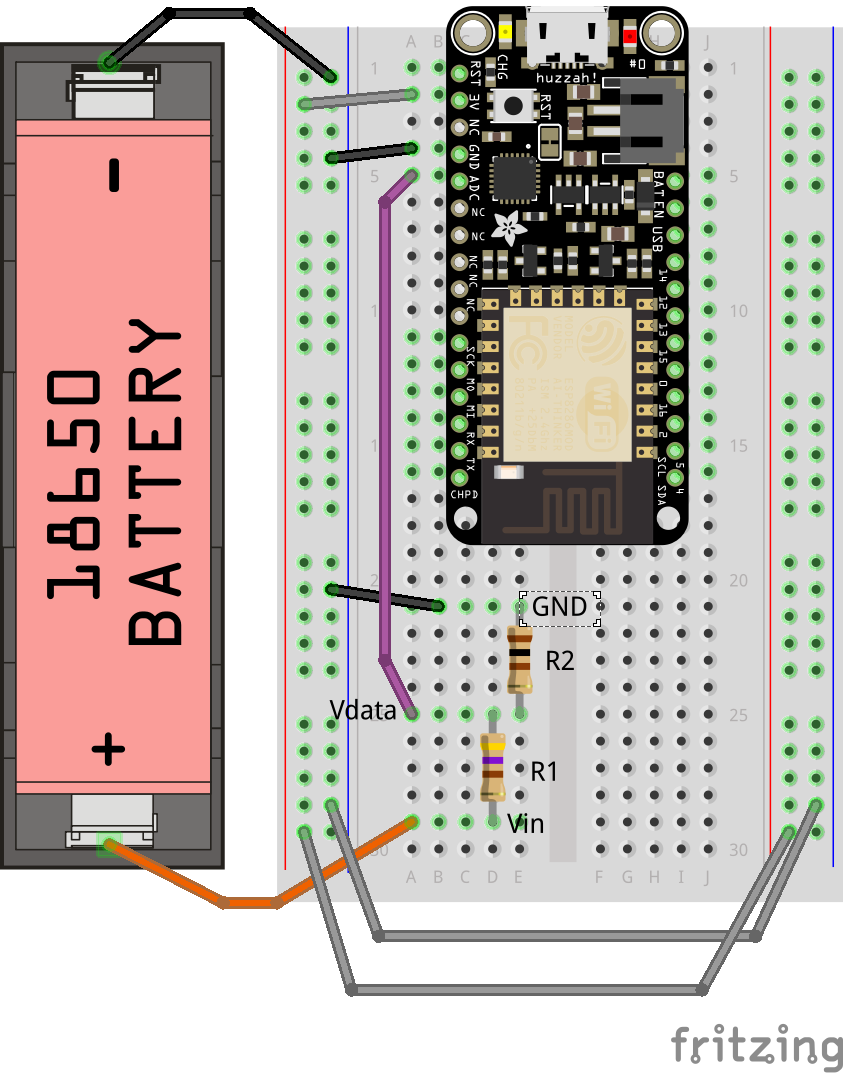
\includegraphics[width=\MFW]{Fritzing/feather_voltage_divider2_bb.png}}{https://publicsensors.org/IntroSensors/Fritzing/feather_voltage_divider2_bb.png}
		\caption[Voltage divider schematic]{An illustration of the layout for an analog voltage sensor, using a \texttt{voltage divider} to measure voltage from an \texttt{\texttt{18650}} battery.
		In the schematic, jumpers that are not needed but may be left in place if already present are indicated in gray.}
		\labfig{feather_voltage_divider2}
	\end{center}
\end{marginfigure}
An example breadboard layout is given in \reffig{feather_voltage_divider2}.

Here's the step-by-step (\underline{be sure to do these in order}):
\begin{enumerate}
	\item \textbf{Select, label and test the resistors $R_1$ and $R_2$.}
	\begin{itemize}
		\item[$\circ$] Choose resistors for the $R_1$ and $R_2$ values you identified as yielding the best voltage divider characteristics.
		\item[$\circ$] Measure the actual resistances using the multimeter.
		\item[$\circ$] Label each resistor with a piece of tape, identifying it as to the role it will play ($R_1$ or $R_2$) and its actual resistance.
	\end{itemize}
	By measuring and labeling, you account for the possibility that the actual resistances differ substantially from the nominal resistances.
	You also reduce the risk that you will accidentally reverse $R_1$ and $R_2$ in your circuit, which could destroy the \adc.

	\item \textbf{Insert your microcontroller in your breadboard, in the standard position.}

	\item \textbf{Insert the resistors into the breadboard.}

	\reffig{feather_voltage_divider2} shows one possible layout, but many variations are possible.
	The key requirements are that:
	\begin{itemize}
		\item[$\circ$] One end of both resistors connect by inserting into the same row.
		\item[$\circ$] The other ends of each resistor insert into otherwise empty rows.
	\end{itemize}
	\textbf{DOUBLE CHECK THAT YOUR $R_1$ AND $R_2$ RESISTORS ARE IN THE CORRECT POSITIONS, AS INDICATED IN \reffig{feather_voltage_divider2}}.

	\item \textbf{Use a jumper to connect the free end of your $R_2$ resistor to the negative rail.}

	\item \textbf{Insert your \texttt{\texttt{18650}} battery into the battery holder, making sure to have the positive terminal of the battery in the positive end of the battery holder.}

	\item \textbf{Insert the ``\texttt{-}'' (black) wire from the battery holder into the negative rail  (\texttt{GND}).}

	\item \textbf{Insert the ``\texttt{+}'' (red) wire from the battery holder to the free end of your $R_1$ resistor  (\texttt{Vin}).}

	\item \textbf{Test your connections!}

	At this point, there is voltage across the voltage divider.
	To insure your circuit is safe for your \adc, confirm that:
	\begin{itemize}
		\item[$\circ$] Voltage across the free ends of $R_1$ and $R_2$ is in the range of \texttt{+3.6} to \texttt{+4.3 volts}.
		\item[$\circ$] Voltage across $R_2$ is in the range of \texttt{0} to \texttt{V\textsubscript{ref}} (\texttt{0} to \texttt{+1 volts} on an \texttt{ESP8266}, \texttt{0} to \texttt{+2.45 volts} on an \texttt{ESP32}, or \texttt{0} to \texttt{+2.5 volts} on an \texttt{ESP32-S2} ).
	\end{itemize}
	\textbf{IF EITHER OF THESE IS NOT TRUE, DO NOT PROCEED UNTIL YOU HAVE IDENTIFIED AND CORRECTED THE PROBLEM}.

	\item \textbf{Use a long jumper to connect your \adc pin to the row with both $R_1$ and $R_2$ connections (\texttt{Vdata}).}
	Unfortunately \texttt{ESP32} and \texttt{ESP32-S2} can only access the ADC on a subset of pins that differ from board to board. This means there is no single diagram can show hookup connections required for all three boards \sidenote[][*]{
	\begin{kaobox}[backgroundcolor=\SNcolor,frametitlebackgroundcolor=\SNcolor,frametitle=Where are the useable \adc pins?]
	 The useable ADC \texttt{gpio} pins for each system, along with the pins these map to on the Feather form factor, are:
	\begin{table}[H]
	\centering \begin{small}
	\begin{tabular}{c c }
		\multicolumn{2}{l}{ESP32} \\
		\hline
		\textbf{\texttt{gpio}}  & \textbf{Feather} \\
		\hline
		34  & A2 \\
		39  & A3 \\
		36  & A4 \\
		33  & 33 \\
		32  & 32 \\
		\hline
	\end{tabular}
	\end{small}
	\end{table}
	\begin{table}[H]
	\centering \begin{small}
	\begin{tabular}{c c }
		\multicolumn{2}{l}{ESP32-S2} \\
		\hline
		\textbf{\texttt{gpio}}  & \textbf{Feather} \\
		\hline
		5  & D5 \\
		6  & D6\\
		8  & A5 \\
		9  & D9 \\
		10  & D10 \\
		\hline
	\end{tabular}
	\end{small}
	\end{table}
	\end{kaobox}
} 

	\item \textbf{Use a jumper to connect your microcontroller's \texttt{GND} pin to the negative rail.}

	When you establish this connection, it insures that the ``zero'' voltage (\texttt{GND}) is the same for the battery, voltage divider and microcontroller.

\end{enumerate}

	The hardware assembly is now complete.
	Now it's time for the software!

\begin{enumerate}[resume]
	\item \textbf{Connect a USB cable to your microcontroller, an open a \texttt{REPL} session.}

	\item \textbf{Create an \adc object, and use it to query the voltage of $V_{data}$.}

	Unfortunately, the syntax and definition of the \texttt{gpio} pin associated with pin A0 differs between \texttt{ESP8266}, \texttt{ESP-32}, and \texttt{ESP32-S2} feather-based microcontrollers.   Snippets are given here for each board, assuming the data pin is connected to the ADC pin indicated.

\textbf{\texttt{ESP8266} Snippet, assuming data pin connected to \texttt{Pin A0}:}
\begin{lstlisting}[language=Python]
from machine import ADC   # import the ADC module
adc = ADC(0)              # create an ADC object
adc.read()    # read the ADC and print the result
\end{lstlisting}

\textbf{\texttt{ESP32} Snippet, assuming data pin connected to \texttt{Pin A2}:}
\begin{lstlisting}[language=Python]
from machine import ADC, PIN   # import the ADC and PIN modules
adc = ADC(Pin(34))            # create an ADC object on gpio26 (Feather pin A0)
adc.read()    # read the ADC and print the result
\end{lstlisting}

\textbf{\texttt{ESP32-S2}  Snippet, assuming data pin connected to \texttt{Pin A5}::}
\begin{lstlisting}[language=Python]
from machine import ADC, PIN   # import the ADC and PIN modules
adc = ADC(Pin(8))            # create an ADC object on gpio8 (Feather pin A5)
adc.read()    # read the ADC and print the result
\end{lstlisting}


	\item \textbf{On your laptop or desktop, write a Micropython function that prints the battery voltage, $V_{in}$.}

	Use the following code to define your function, replacing the example resistor values with the correct values for your voltage divider:

\begin{lstlisting}[language=Python]
from machine import ADC, Pin
try:
    adc = ADC(0)
except:
    adc = ADC(Pin(8))
    adc.atten(ADC.ATTN_11DB)
def battery_voltage(adc, Cmax, Vref,R1=470., R2=47.):
    vdata=adc.read()/Cmax*Vref
    vin = vdata*(R1+R2)/R2
    return vin
\end{lstlisting}


	\item \textbf{Execute your function on your microcontroller.}

	You can load this function either using the \texttt{<ctrl>-e/<ctrl>-d} sequence to paste it into a \texttt{REPL} session, or by transferring the file and importing it.
	Either way, the commands (with resistor values modified)
\begin{lstlisting}[language=Python]
from BatteryVoltage import battery_voltage
battery_voltage(R1=470.,R2=47.)
\end{lstlisting}
	should now return a measurement of your \texttt{\texttt{18650}} battery voltage.
	If you change to other resistor values, you can calculate voltage for the new voltage divider by changing the \texttt{R1} and \texttt{R2} arguments of the function.
\end{enumerate}

\loadMilestone{mlst:04b} % load milestone with tags id: mlst:04b

%\vspace{3 cm}
%\begin{itemize}
%	\item Quantities and units
%	\item Analogies with pipe flow
%	\item Ohm's Law
%	\item voltage-based analog sensors: thermistors
%	\item time-based analog sensors: sonar \& light
%\end{itemize}
%
%\begin{itemize}
%	\item multimeters
%	\item ADC on ESP8266
%	\item how-to: design a voltage divider
%	\item how-to: build a voltage divider
%\end{itemize}
\newpage

\subsection{Calibrating maximum voltage of ADC}

So far, we've assumed that the specifications for your microcontroller allow you to know, with great precision, the voltage $V_{ref}$ that is associated with the maximum count $C_{max}$ on your microcontroller.
However, this value can vary from \texttt{ESP} board to \texttt{ESP} board, even within a given model.
For precise measurements to be possible, this value should be known to more than the one or two significant digits provided in the manufacturer's documentation.
  
\begin{marginfigure}[-5cm]
	\begin{center}
		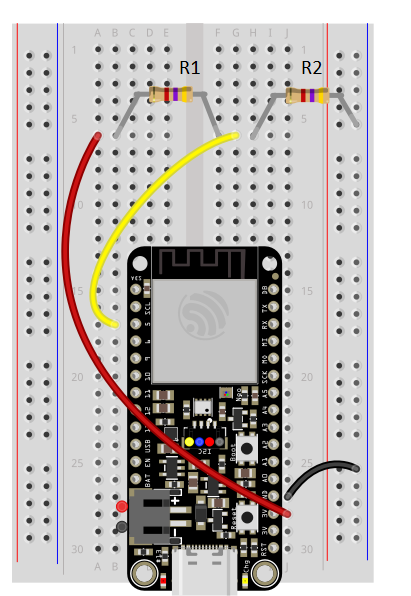
\includegraphics[height=7cm]{Images/check_vref2.png}
		\caption[Checking reference voltage]{Circuit for checking the internal reference voltage for \adc.}
		\labfig{vref}
	\end{center}
\end{marginfigure}

Thankfully, it's straightforward to use the circuit you developed for measuring battery voltage, in combination with the 3.3V power supply for your device, to develop this estimate. To accomplish this, set up a voltage divider on a breadboard (\reffig{vref}), with the high voltage to the voltage divider coming out of the \texttt{3.3V} pin. Feather-based breakout boards provide a fairly stable voltage on this pin that should be quite close to \num{3.3} \si{\volt} (although feel free to measure this with a multimeter set to the DC voltage setting).  Use resistors that divide this down so that the voltage $V_{data}$ is known.  Once a measurement is made, we can now compute the internal reference voltage using the simple relationship

	\begin{equation}\label{voltage_ratio}
		\frac{V_{data}}{V_{ref}} = \frac{C_{ADC}}{C_{max}}
	\end{equation}

where $C_{ADC}$ is the actual count returned by the \adc. Using the known value of $V_{data}=3.30 R2/(R1+R2)$, it is straightforward to solve for $V_{ref}$,

	\begin{equation}\label{vref}
		V_{ref} = 3.30\frac{R2}{R1+R2}\frac{C_{max}}{C_{ADC}}
	\end{equation}

This can be solved programmatically using the following code, although note that pin assignments may need to be adjusted to match the specific ADC pin being used in your implementation.

\begin{lstlisting}[language=Python]
#import libraries
import machine
from machine import Pin, ADC
import time

#specify parameters
n = 20 #number of samples to average
R1 = 10000
R2 = 10000
v33 = 3.30
#compute v_data
v_data = 3.3*R2/(R1+R2)

#initialize ADC
try:
    #works for ESP8266
    adc = ADC(0)
    maxcount = 1023
except:
    #works for ESP32
    adc = ADC(Pin(5))
    adc.atten(ADC.ATTN_11DB)
    maxcount = 8191  #4095 if ESP32

#Collect n measurements, average, and print results
total = 0
for i in range(20):
    total = total + adc.read()
    time.sleep(0.2) #necessary to give ADC time to reset
c_adc_av = total / n 
v_ref = v_data * maxcount / c_adc_av
print(f"n = {n}, average ADC count = {c_adc_av}, average Vref = {v_ref}")
\end{lstlisting}


\section{Environmental sensing with voltage: measure temperature with a thermistor}
\labsec{cal_therm}
A \htmladdnormallink{thermistor}{https://en.wikipedia.org/wiki/Thermistor} is an electrical component whose resistance changes with temperature.
Thermistors are readily available and inexpensive, and low cost temperature sensors made from them can have very good accuracy and precision.
Unsurprisingly, thermistors are widely used as temperature sensors in industry and household appliances.
For example, the temperature in refrigerators and ovens are often controlled by circuits using a thermistor to sense temperature.
In this section you will design, assemble and calibrate an analog sensor using a thermistor, and use it to measure variations in environmental temperature.

The voltage divider you built in \refsec{meas_volt} was designed to measure voltage from a battery. % that was outside the \texttt{ESP8266} \adc's tolerance limits.
In the design process, you used Ohm's Law to deduce the unknown voltage, $V_{in}$, from a known pair of resistors $R_1$ and $R_2$ and the measured output voltage, $V_{data}$.
As Equation \ref{OhmsRVI} shows, Ohm's Law has an equivalent application in deducing resistance from known voltage and current.
This suggests that, in a voltage divider where $V_{in}$ and either $R_1$ or $R_2$ are known, $V_{data}$ could be used to infer the other, unknown resistor value.
%This suggests that a voltage divider in which both $V_{in}$, $V_{data}$ and either $R_1$ or $R_2$ are known could be used to infer the other, unknown resistor value.

The analog temperature sensor you will make uses a voltage divider in this way.
The unknown resistor in this voltage divider will be a thermistor.
Quantifying this thermistor's resistance --- combined with a calibration of how its resistance varies as a function of temperature --- will enable you to use your microcontroller to measure ambient temperature.

Using Equation \ref{vd4} as a starting point, we have two options.
We could use the thermistor to replace $R_1$.
In that case, solving Equation \ref{vd4} for $R_1 = R_{therm}$ gives us
\begin{equation}\label{therm1}
R_{therm} = \frac{V_{in}-V_{data}}{V_{data}}R_2.
\end{equation}
Alternatively, we could use the thermistor to replace $R_2$.
Then, solving Equation \ref{vd4} for $R_2 = R_{therm}$ gives us
\begin{equation}\label{therm2}
R_{therm} = \frac{V_{data}}{V_{in}-V_{data}}R_1.
\end{equation}
We do not know ahead of time which strategy will yield a better temperature sensor.
Which resistor to replace, and what value to choose for the remaining resistor, will emerge from the sensor design process.

\subsection{Thermistor temperature-resistance curves}
Thermistors are usually referred to by their \texttt{nominal resistance value}, which is their designed resistance at the reference temperature, $25^\circ$ \texttt{C} ($77^\circ$ \texttt{F}).
Common nominal resistance values for thermistors range from $100\Omega$ through $100k\Omega$.
Within this range are many nominal resistance values that are somewhat standard for specific purposes.
For example, many 3D printers use a $22k\Omega$ thermistor to measure the temperature at which melted plastic is being extruded to build up a part.

The most common type of thermistor in temperature sensors is a \texttt{``negative temperature coefficient''} (\texttt{NTC}) thermistor.
In an \texttt{NTC} thermistor, the resistance is lower at higher temperatures, and higher at lower temperatures.
(The converse --- a \texttt{``positive temperature coefficient''} or \texttt{PTC} thermistor, has higher resistance at higher temperatures, and lower resistance at lower temperatures.)
This change in resistance with temperature is what makes a thermistor suitable as the basis of a temperature sensor.
However, it also means that we must anticipate the entire range of possible resistance values in our circuit design, to get the best possible resolution while insuring that the voltage divider will never exceed the \adc voltage tolerance.

%To evaluate alternative configurations for a voltage divider measuring thermistor resistance, we need to consider how that resistance varies over the relevant range of temperatures.
%\texttt{NTC} means that resistance goes down with increasing temperature.
A systematic study of temperature-resistance curves for \texttt{NTC} thermistors was published in 1968 by Steinhard and Hart \cite{STEINHART1968497}.
The formula that they found to best describe these curves is known as the \htmladdnormallink{\texttt{Steinhart-Hart equation}}{https://en.wikipedia.org/wiki/Steinhart\%E2\%80\%93Hart\_equation},
\begin{equation}\label{therm3}
\frac{1}{T_{k}} = A + B \ln R_{th} + C (\ln R_{th})^3.
\end{equation}
In this equation, $T_{k}$ is thermistor temperature in \texttt{kelvins}.
$R_{th}$ is resistance in \texttt{ohms}.
$A$, $B$ and $C$ are calibration constants --- called \texttt{Steinhart-Hart coefficients} ---  that are determined for a given thermistor by measuring its resistance at three known temperatures.
If the three calibration temperatures are $T_{k,1}$, $T_{k,2}$ and $T_{k,3}$, and the corresponding resistances are $R_1$, $R_2$ and $R_3$, then the following formulas determine $A$, $B$ and $C$:
\begin{eqnarray}
L_1 = \ln R_1, ~L_2 = \ln R_2, ~L_3 = \ln R_3  \non \\
Y_1 = \frac{1}{T_{k,1}}, ~Y_2 = \frac{1}{T_{k,2}}, ~Y_3 = \frac{1}{T_{k,3}} \non \\
\gamma_2 = \frac{Y_2-Y_1}{L_2-L_1}, \gamma_3 = \frac{Y_3-Y_1}{L_3-L_1} \non \\
C = \frac{\gamma_3-\gamma_2}{L_3-L_2} (L_1+L_2+L_3)^{-1}  \label{therm4}\\
B = \gamma_2 - C(L_1^2 + L_1 L_2 + L_2^2) \non \\
A = Y_1 - (B+L_1^2 C) L_1 \non
\end{eqnarray}
It's sometimes useful to calculate a thermistor's resistance, $R_{th}$, from its temperature (that is, the \emph{inverse} of Equation \ref{therm3}).
One approach is through trial and error --- plugging a few guesses of $R_{th}$ into Equation \ref{therm3}), it's usually possible to come quite close to a specific $T_k$.
However, an explicit formula is available:
\begin{equation}\label{therm5}
R_{th} = e^{\left(\sqrt[3](y-x) - \sqrt[3](y+x)\right)} ,
%R_{th} = \exp\left(\sqrt[3](y-x) - \sqrt[3](y+x)\right) ,
\end{equation}
where
\begin{equation}\label{therm6}
x = \frac{1}{2C} \left( A - \frac{1}{T_{k}} \right), ~ y = \sqrt{\left(\frac{B}{3C}\right)^3+x^2}.
\end{equation}
These formulas provide the theoretical basis for calibrating your thermistor.

%http://www.aetsolar.com/literature/Manuals/TempVsResistChart.pdf

\subsubsection{\howto Calibrate a thermistor}
\labsec{therm_cal}
The first step in designing a thermistor-based temperature sensor is to calibrate its temperature-resistance curve by determining its Steinhart-Hart coefficients.
In this section, you will create simple water baths at three known temperatures $T_{k,1}$, $T_{k,2}$ and $T_{k,3}$, and use them to measure thermistor resistances $R_1$, $R_2$ and $R_3$ in Equation \ref{therm3}.

You will then use Equations \ref{therm3}--\ref{therm6} to calculate the Steinhart-Hart coefficients for your thermistor.
Establishing the Steinhart-Hart coefficients calibrates your thermistor, enabling you to calculate temperature from resistance and \textit{vice versa}.

It's worth noting that, to be good calibration temperatures, $T_{k,1}$, $T_{k,2}$ and $T_{k,3}$ should span all or most of the temperature range of interest.
Furthermore, they should ideally be spaced roughly equally apart within this range.
This is so that, to the extent possible, the Steinhart-Hart equations will be used to \texttt{interpolate} rather than \texttt{extrapolate} the temperature-resistance relationship.
As you may have found in previous scientific work, extrapolation often magnifies small errors in calibration such that they become disproportionately large far from measured data points.

In the calibration procedure below, we will illustrate the steps using example values from a $10k\Omega$ thermistor.
Substitute the values you obtain from your thermistor into these calculations.
\begin{enumerate}
	\item \textbf{Prepare water baths at three different temperatures.}

	Typically, most laboratory thermometers give temperature in $^\circ$ \texttt{Celsius}.
	Remember that temperature in Celsius, $T_c$, is related to $T_k$ by
	\begin{equation*}
		T_k = T_c + 273.15, ~T_c = T_k - 273.15.
	\end{equation*}
	To use water bath temperatures measured in \texttt{Celsius} for thermistor calibration, you must either convert them to $^\circ$ \texttt{Kelvin} using the formula above, or use the version of the Python scripts below that does that conversion for you.

	\smallskip
%	To be good calibration temperatures, $T_{k,1}$, $T_{k,2}$ and $T_{k,3}$ should span all or most of the temperature range of interest, and be spaced roughly equally apart within this range.
	In most classrooms and laboratories, three suitable temperatures that are easy to produce in water baths are:
	\begin{itemize}
		\item[$\circ$] $0^\circ$ \texttt{C}, which is the equilibruim temperature of a mixture of frozen and liquid fresh water.
		\item[$\circ$] $100^\circ$ \texttt{C}, which is the boiling temperature of fresh water.
		\item[$\circ$] Room temperature, which is usually close to $25^\circ$ \texttt{C}.
%  Human body temp: $36.5–37.5^\circ$ \texttt{C}
	\end{itemize}

	A good way to create ``water baths'' at these three temperatures for thermistor calibration is with paper bowls or cups, filled with a water/ice mixture, boiling water and room temperature water.
	Cover each bath with a lid, so that it maintains its temperature for longer and does not cool through evaporation.
	Confirm the actual temperatures of your water baths with the most accurate thermometer you can find, e.g. by inserting it through a small hole in the lid.

	\item \textbf{Prepare your thermistor for resistance measurements.}

	The goal in this step is to enable you to measure resistance across the thermistor with a multimeter, while that thermistor is held at known temperatures by the water baths.
	We leave it to your ingenuity to come up with effective, creative solutions to the materials you have on hand.

	\smallskip
	%We'll illustrate with two examples, both of which are inexpensive and easily obtained $10k\Omega$ thermistors.\todo{pictures of Thermistors A and B}
	%However, many other thermistor types and water bath arrangements are workable.
	Handling thermistors experimentally depends on their thermal mass and waterproofing.  Consider two models of thermistor, one, \texttt{Thermistor A}, that is just the bare thermistor, and the other, \texttt{Thermistor B}, that has been waterproofed by its manufacturer.
	\begin{itemize}
		\item[$\circ$] \texttt{Thermistor A} is a ``bead'' thermistor, with two bare wires.
		This kind of thermistor responds quickly to temperature changes, but is not protected from water or other corrosive or conductive liquids.

		\smallskip
		To calibrate \texttt{Thermistor A}, use removable tape (like painter's masking tape) to attach it snugly to the outside of the water baths
		It should directly touch the surface of the water bath, to conduct heat as quickly as possible from the water bath surface.
		Then, cover the thermistor with a layer of foam or folded paper towels to insulate it from the surrounding air.
		Keep in mind that the wires can conduct heat into or out of the thermistor, so ideally they will also be in contact with the bath and covered by the insulation.
		%Be sure, though, to leave enough of the wires exposed to connect to multimeter leads to measure resistance.

		\item[$\circ$] \texttt{Thermistor B} is ``potted'', meaning it is encased in a protective stainless steel sleeve, and embedded in epoxy or some other sealant.
		This casing means that the thermistor is waterproof --- it can be submerged directly into the water baths.
		However, because the casing retains a significant amount of heat, potted sensors can be slower to respond to temperature changes than bead thermistors.

		\smallskip
		To calibrate \texttt{Thermistor B}, immerse the thermistor entirely within the water bath, with its wires coming out through a small hole in the lid.

	\end{itemize}

	\item \textbf{Measure resistance at each water bath temperature with a multimeter.}

	In making these measurements, keep in mind:
	\begin{itemize}
		\item[$\circ$] The \texttt{equilibration time} of the thermistor.
		This is the time it takes for the interior of the thermistor to equalize in temperature with the surface of the water bath.
		You can get an estimate of the equilibration time by watching the resistance measured on a multimeter change immediately after you place the thermistor in contact with a surface of different temperature.
		Typical equilibration times range from a few seconds to several minutes.
		\item[$\circ$] %Multimeters also have internal equilibration times.
		Some multimeters have a significant amount of measurement noise, especially for very low or very high resistance values.
		When making your measurements, wait until the resistance value appears to stabilize.
		Then, record the resistance value at five times, spaced several seconds apart.
		Take the median of these as the most accurate resistance measurement.
	\end{itemize}

	\item \textbf{Calculate the Steinhart-Hart coefficients.}

	The Python functions below enable you to calculate the Steinhart-Hart coefficients for your thermistor.
	To use them, substitute your measured temperature and resistance values for the default \texttt{T}'s and \texttt{R}'s.
	You may run these functions on your computer or, using the \texttt{<ctrl>-e / <ctrl>-d} technique, copy and run them on your microcontroller.

	\smallskip
	Use \lstinline{SH_coeffs_kelvins} if your temperatures are in $^\circ$\texttt{Kelvin}, and \lstinline{SH_coeffs_celsius} if your temperatures are in $^\circ$\texttt{Celsius}. Both functions return the Steinhart-Hart coefficients \lstinline{(A, B, C)} as a Python tuple.
	\lstinputlisting[language=Python,label=SteinhartHart,caption={\htmladdnormallink{\texttt{SteinhartHart.py}}{https://github.com/publicsensors/IntroSensors/blob/main/Codes/SteinhartHart.py}: Python functions to calculate Steinhart-Hart coefficients for thermistor calibration.}]{Codes/SteinhartHart.py}


	\item \textbf{Verify the resistor and temperature calculations.}

	The Python functions below calculate temperature from resistance and \textit{vice versa} for a calibrated thermistor.
	\lstinputlisting[language=Python,label=thermistor,caption={\htmladdnormallink{\texttt{thermistor.py}}{https://github.com/publicsensors/IntroSensors/blob/main/Codes/thermistor.py}: Python functions to calculate temperature from resistance and \textit{vice versa} for a calibrated thermistor.}]{Codes/thermistor.py}
	As an initial test, try calculations with your known values: $R_1$ from $T_{k,1}$, $T_{k,2}$ from $R_2$, \etc
	For \emph{consistency}, you should get the same result as you entered for your calibration.

	\smallskip
	Next, use both a thermometer and your thermistor to measure another temperature, e.g. outside or in an unheated storage space, or in a water bath at a new temperature.
	What is the percent error between the thermometer and your thermistor temperature readings?

\end{enumerate}
\loadMilestone{mlst:04c} % load milestone with tags id: mlst:04c


\subsection{Thermistor circuit design}
To design a circuit that effectively uses a thermistor to measure environmental temperatures, you will use the tools you developed in the last two sections: A calibration enabling you to calculate your thermistor's resistance across the relevant range of temperatures, and a spreadsheet enabling you to calculate which resistor combinations satisfy your microcontroller's \adc voltage tolerance.

There are two circuit configurations that you need to consider:
\begin{itemize}
	\item Configuration 1, in which the thermistor replaces resistor $R_1$ from the voltage divider circuit:
	\begin{figure}[H]
		\centering
%	\begin{center}
		\begin{tikzpicture}[american voltages]
		\draw
		(0,0) to [short,l=$V_{in}$, *-] (1,0)
		to [thRn, l=$RTH_1$] (3,0)
		to [short, i_=$I$,l=$V_{data}$] (4,0)
		to [R, l=$R_2$] (6,0)
		to [short,l=GND, -*] (7,0);
		\end{tikzpicture}
		\caption[Thermistor circuit \#1]{Schematic diagram of a voltage divider circuit, with the thermistor replacing resistor $R_1$.}
		\labfig{therm_cir1}
%	\end{center}
	\end{figure}

	\item Configuration 2, in which the thermistor replaces resistor $R_2$ from the voltage divider circuit:
	\begin{figure}[H]
		\centering
%	\begin{center}
		\begin{tikzpicture}[american voltages]
		\draw
		(0,0) to [short,l=$V_{in}$, *-] (1,0)
		to [R, l=$R_1$] (3,0)
		to [short, i_=$I$,l=$V_{data}$] (4,0)
		to [thRn, l=$RTH_2$] (6,0)
		to [short,l=GND, -*] (7,0);
		\end{tikzpicture}
		\caption[Thermistor circuit \#2]{Schematic diagram of a voltage divider circuit, with the thermistor replacing resistor $R_2$.}
		\labfig{therm_cir2}
%	\end{center}
	\end{figure}
\end{itemize}
In these circuit diagrams, the box with the diagonal line represents the thermistor, in which resistance is modulated by temperature. We have labeled the thermistor in these positions $RTH_1$ and $RTH_2$, to remind us that these thermistors replace resistors $R_1$ and $R_2$, respectively, in our voltage divider calculations.

\subsubsection{\howto Design a voltage divider for a thermistor}
\labsec{therm_des}
\begin{enumerate}
	\item \textbf{Make two copies of the voltage divider calculations spreadsheet from \refsec{vd_design}.}

	Save one with a name that includes something like ``\texttt{RTH1}''. You'll use this one to make calculations for Configuration 1.
	Likewise, save the other with an informative name that includes something like ``\texttt{RTH2}''.

	\item \textbf{Modify the \texttt{RTH1} spreadsheet for the thermistor circuit.}

	Starting with the voltage divider spreadsheet:
	\begin{itemize}
		\item[$\circ$] \textbf{Change the entries under the \texttt{Vin} column heading to \texttt{3.3}.}
		This reflects the fact that we will use the \texttt{3V3} pin to power the thermistor circuit. This pin always outputs exactly \texttt{3.3 volts}.

%		\item[$\circ$] Change the logical test in the fifth column to read \lstinline{R2<=R1/2.3?}. Then, change the formula in the rest of the fifth column to read \lstinline{=C2<(B2/2.3)}. This reflects the criterion on resistances to meet the voltage tolerance with the $V_{in}=3.3$ \texttt{volts}.
%
		\item[$\circ$] \textbf{In the top row, change the \texttt{R1} column header to \texttt{RTH1}.}

		For neatness, make the same change in the \texttt{R2/R1} header, to \texttt{R2/RTH1}.
		\item[$\circ$] \textbf{In the top row under the \texttt{RTH1} column header, enter the thermistor resistance you measured at the lowest temperature, $0^\circ$\texttt{C}.}
		\item[$\circ$] \textbf{In the next row, replace the \texttt{RTH1} column resistance with the thermistor resistance you measured at the highest temperature, $100^\circ$\texttt{C}.}
		These represent the whole range of resistances that can occur in the voltage divider within the calibrated interval, $0-100^\circ$\texttt{C}.

		\item[$\circ$] \textbf{Copy a candidate $R_2$ resistor value into \underline{both} rows under the \texttt{R2} column.}

		Your spreadsheet rows will then look something like this (using $R_2=100\Omega$ resistors as an example):
\begin{table}[H]
	\centering
	\begin{small}
		\begin{tabular}{|c|c|c|c|c|c|c|c|c|}
		\hline
			\textbf{A}  & \textbf{B} & \textbf{C} & \textbf{D} & \textbf{E} & \textbf{F} & \textbf{G} & \textbf{H} & \textbf{I} \\
			\hline
			Vin  & RTH1 & R2 & R2/RTH1 & Vdata & Vdata<1? & I & W & Vres \\
			\hline
			3.3 & 32648  & 100 & 3.06E-03 & 1.01E-02 & TRUE & 1.01E-04 & 3.33E-04 & 3.20E-01 \\
			\hline
			3.3 & 680  & 100 & 1.47E-01 & 4.23E-01 & TRUE & 4.23E-03 & 1.40E-02 & 7.62E-03 \\
			\hline
		\end{tabular}
	\end{small}
\end{table}

%		\item[$\circ$] \textbf{Examine the results in the remaining }

	\end{itemize}


	\item \textbf{Calculate ``self-heating'' of the thermistor due to dissipated electrical energy.}

	In the ``\texttt{W}'' column of your spreadsheet, you calculate the rate at which electrical power is lost to heat in the voltage divider.
	This is an important piece of information, because high rates of power dissipation can discharge the battery faster than necessary.

	\smallskip
	In our thermistor circuit, however, power dissipated to heat plays another role --- it heats the temperature sensor!
	If the thermistor itself is generating a substantial amount of heat, that could cause artifacts in its temperature readings.

	\smallskip
	To calculate the heat generation inside the thermistor, $W_{th}$, we can again use Equation \ref{watts}.
	Because we have already calculated the current, $I$, the simplest approach is to calculate $W_{th}$ as the product of $I^2$ and thermistor resistance.
\begin{itemize}
	\item[$\circ$] \textbf{Add a column header, \texttt{WTH1}, in the column after \texttt{Vres}.}
	\item[$\circ$] \textbf{Enter the formula \lstinline{=(H2^2)*B2} into the cells below \texttt{WTH1}.}
\end{itemize}
	Your spreadsheet will now look something like this:
\begin{table}[H]
	\centering
	\begin{small}
		\begin{tabular}{|c|c|c|c|c|c|c|c|c|c|}
			\hline
			\textbf{A}  & \textbf{B} & \textbf{C} & \textbf{D} & \textbf{E} & \textbf{F} & \textbf{G} & \textbf{H} & \textbf{I} & \textbf{J} \\
			\hline
			Vin  & RTH1 & R2 & R2/RTH1 & Vdata & Vdata<1? & I & W & Vres & WTH1\\
			\hline
			3.3 & 32648  & 100 & 3.06E-03 & 1.01E-02 & TRUE & 1.01E-04 & 3.33E-04 & 3.20E-01 & 3.32E-04\\
			\hline
			3.3 & 680  & 100 & 1.47E-01 & 4.23E-01 & TRUE & 4.23E-03 & 1.40E-02 & 7.62E-03 & 1.22E-02\\
			\hline
		\end{tabular}
	\end{small}
\end{table}
	where the last column is the heat (in \texttt{watts}) generated in the thermistor.

	\item \textbf{Explore alternative resistor values, by making copies of the two rows of calculations, and entering different values for \texttt{R2}.}

	Does the new resistance value satisfy the \adc voltage tolerance?\sidenote[][*12]{
		\begin{kaobox}[backgroundcolor=\SNcolor,frametitlebackgroundcolor=\SNcolor,frametitle=Resist-metic]As we found in the voltage divider discussion, the total resistance of two resistors connected in \emph{series} (one connected end to end with the other) is simply the sum of their individual resistances: $R_{total}=R_1+R_2$.
			You can use this fact if you want to use a resistor value that you don't have in hand.
			For example, if you have $510\Omega$ and $220\Omega$ resistors, you can attach them in series to form a $510+220=730\Omega$ resistor.
		\end{kaobox}
	}
	Is the resolution better or worse with new \texttt{R2} resistances?
	Are the total power dissipation and the heat generated inside the thermistor larger or smaller than the previous \texttt{R2} choices?

	\item \textbf{Repeat all the above steps for the \texttt{RTH2} spreadsheet, but this time replacing \texttt{R2} with \texttt{RTH2}.}

	In this case, the formula for \texttt{WTH2} is \lstinline{=(H2^2)*C2}.
	The result (using $R_1=100k\Omega$ as an example) will be similar to:
\begin{table}[H]
	\centering
	\begin{small}
		\begin{tabular}{|c|c|c|c|c|c|c|c|c|c|}
			\hline
			\textbf{A}  & \textbf{B} & \textbf{C} & \textbf{D} & \textbf{E} & \textbf{F} & \textbf{G} & \textbf{H} & \textbf{I} & \textbf{J} \\
			\hline
			Vin  & R1 & RTH2 & RTH2/R1 & Vdata & Vdata<1? & I & W & Vres & WTH2\\
			\hline
			3.3 & 1.00E+05  & 32648 & 3.26E-01 & 8.12E-01 & TRUE & 2.49E-05 & 8.21E-05 & 9.37E-03 & 2.02E-05\\
			\hline
			3.3 & 1.00E+05  & 680 & 6.80E-03 & 2.23E-02 & TRUE & 3.28E-05 & 1.08E-04 & 1.45E-01 & 7.31E-07\\
			\hline
		\end{tabular}
	\end{small}
\end{table}

\end{enumerate}
\loadMilestone{mlst:04d} % load milestone with tags id: mlst:04c


\subsection{Thermistor circuit assembly and programming}
Laying out and assembling a voltage dividing circuit to measure temperature with a thermistor requires only a few changes from the voltage divider you built in \refsec{vd_assem}.
Then, measuring temperature involves three steps that happen in Python scripts:
\begin{itemize}
	\item Use the \adc to measure $V_{data}$.
	\item Use Equation \ref{therm1} or \ref{therm2} (depending on your circuit configuration) to infer the thermistor resistance $R_{therm}$ from $V_{data}$.
	\item Use your thermistor calibration from \refsec{therm_cal} to infer temperature from $R_{therm}$.
\end{itemize}
The following \textit{HOW-TO} takes you through these steps.

\subsubsection{\howto Build and test a thermistor circuit}
If you have chosen Configuration 2, your circuit layout will be similar to \reffig{feather_thermistor}.
If you have chosen Configuration 1, your circuit layout will have the thermistor in position \texttt{R1} rather than \texttt{R2}, but be otherwise similar to \reffig{feather_thermistor}.

\labsec{therm_build}
\begin{marginfigure}[-8cm]
	\begin{center}
		\htmladdnormallink{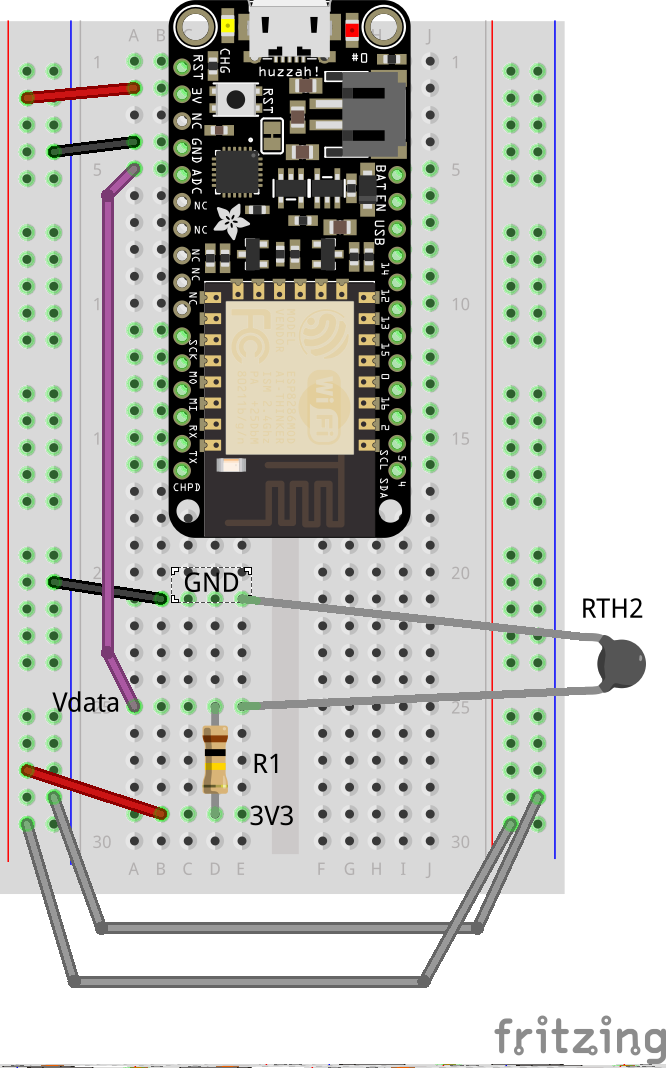
\includegraphics[width=\MFW]{Fritzing/feather_thermistor_bb.png}}{https://publicsensors.org/IntroSensors/Fritzing/feather_thermistor_bb.png}
		\caption[Thermistor circuit schematic]{An illustration of the layout for a circuit using a thermistor to measure temperature.
		This schematic represents Configuration 2, in which the thermistor (here labeled \texttt{RTH2}) takes the place of resistor $R_2$ in the original voltage divider circuit.
		In Configuration 1, the thermistor would instead take the place of resistor $R_1$.
		In the schematic, jumpers that are not needed but may be left in place if already present are indicated in gray.}
		\labfig{feather_thermistor}
	\end{center}
\end{marginfigure}
\begin{enumerate}
	\item \textbf{Disconnect your microcontroller from USB power.}

	\item \textbf{If you are modifying the battery voltage circuit, disconnect one end of the jumper to the \adc.}

	Both these precautions are to prevent accidentally exposing your \adc to voltages higher than its tolerance, while you build and check your circuit.

	\item \textbf{Assemble and double check the thermistor circuit.}

Compared to the battery voltage circuit, the changes are:
	\begin{itemize}
		\item[$\circ$] Use a jumper to connect the power rail to the open end of resistor \texttt{R1} (or \texttt{RTH1} if you are using Configuration 1).

		The power rail, which is connected to the \texttt{ESP8266}'s \texttt{3V3} pin, supplies positive voltage (instead of the battery in the original circuit).
		\item[$\circ$] \textbf{Replace the appropriate resistor (\texttt{R1} for Configuration 1, \texttt{R2} for Configuration 2) with the thermistor.}
		\item[$\circ$] \textbf{Replace the other resistor (\texttt{R2} for Configuration 1, \texttt{R1} for Configuration 2) with the resistor you chose in your design analysis in \refsec{therm_des}.}
	\end{itemize}

	\item \textbf{With the \adc jumper still disconnected, plug the microcontroller into USB power.}

	\item \textbf{Use a multimeter to check that voltage $0 \le V_{data} \le 1$.}

	At this point, the voltage divider should be powered up and operating as it would during temperature measurements.

	\smallskip
	IMPORTANT: IF USING AN \texttt{ESP8266}, IF THE CONDITION $0 \le V_{data} \le 1$ IS NOT MET, STOP AND DEBUG YOUR CIRCUIT.

	\smallskip
	Do not proceed until you've diagnosed and fixed the problem in the circuit --- it could destroy the \adc.

	\item \textbf{Connect the \adc-\texttt{Vdata} jumper.}

\end{enumerate}
That's it for the hardware.
Now for the software!

\begin{enumerate}[resume]
	\item \textbf{Make a copy of the Python script }\lstinline{BatteryVoltage.py} \textbf{from \refsec{vd_assem}, and save it with an informative name such as as }\lstinline{ThermResist.py}\textbf{.}

	\item \textbf{Modify this script so that it calculates thermistor resistance.}

	The necessary changes are:
	\begin{itemize}
		\item[$\circ$] Change the name of the \lstinline{battery_voltage} function to an informative name, e.g. \lstinline{therm_resistRTH2} if you are using Configuration 2.

		\item[$\circ$] \textbf{Change the \texttt{arguments} of the function from the parameters in the original voltage divider,} \lstinline{R1=470.,R2=47.}\textbf{, to the parameters in the thermistor circuit:} \lstinline{R1=1.e5,vin=3.3}\textbf{.}

		\item[$\circ$] \textbf{Replace the calculation of $V_{in}$ in line 4, with calculation of \texttt{RTH1} or \texttt{RTH2} from Equation \ref{therm1} or \ref{therm2}.}

		\item[$\circ$] Replace \texttt{vin} in the \texttt{return} statement with \texttt{RTH1} or \texttt{RTH2}.
	\end{itemize}

	\item \textbf{Save your changes, copy onto your microcontroller, and test the script.}

	To test, call the function with the resistor value that corresponds to your circuit,
\begin{lstlisting}[language=Python]
rth2=therm_resistRTH2(R1=1.e5,vin=3.3)
T=thermistor_temp_celsius(Rth=rth2,A=0.,B=0.,C=0.)
print('Thermistor temperature = ',T)
\end{lstlisting}
	In the call to the \lstinline{thermistor_temp_celsius} function, remember to assign the correct values to $A$, $B$ and $C$ according to the calibration you obtained in \refsec{therm_cal}.


\end{enumerate}
\loadMilestone{mlst:04e} % load milestone with tags id: mlst:04e

%
%\vspace{4cm}
%\begin{itemize}
%	\item temperature-resistance curves
%	\item measuring resistance with a voltage divider
%	\item design and assembly of a thermister-based voltage divider
%	\item calibration and coding for thermister-based temperature measurements
%	\item refining the thermistor circuit using Kirchhoff's Law's
%\end{itemize}


\section{Environmental sensing with voltage: measuring electrical conductivity}
\labsec{ec}
The \emph{electrical conductivity} (\texttt{EC}) of a substance represents its ability to transmit electrical current. For solids, metals are generally good conductors, with copper and aluminum being some of the best. However, it also turns out that other solid substances, including graphite, are conductive.  To confirm this, try connecting a multimeter set to measure resistance across both ends of a broken pencil.  If your multimeter makes good contact with the "lead" (really a graphite/clay mixture), you should see that the total resistance across an entire pencil is only a few \si{\ohm}. 

Fluids can also conduct electricity to varying degrees. Some, like air, are particularly poor conductors that are usually referred to as insulators. Water, on the other hand, can be quite conductive, which is why we all know that it's a bad idea leave powered electrical appliances out in the rain.  The \texttt{EC} of water varies greatly with the concentration of dissolved electrolytes (salts). For this reason, \texttt{EC} measurements are often used to characterize water quality, and \texttt{EC} measurements frequently form the basis of measurements of the salinity of sea water. 

\begin{marginfigure}[-5cm]
	\begin{center}
		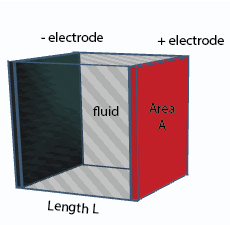
\includegraphics[height=5cm]{Images/ec_cell.png}
		\caption[Ideal EC cell]{An idealized electrical conductivity test cell. Current flows from one charged electrode to the other along a path of length $L$.}
		\labfig{ec_cell}
	\end{center}
\end{marginfigure}

\texttt{EC} is defined as the ability of a fixed volume of substance to transmit current in a single direction. A ideal conductivity measurement cell for a liquid substance might consist of a two planar electrodes, each having the surface area $A$ in contact with the liquid (\reffig{ec_cell}). A perfect insulator would surround the prismatic region, so when one electrode is charged to a higher voltage than the other, all current would flow directly from electrode to electrode by following a single path length $L$.  Conductivity $\kappa$ is defined as 

\begin{equation}\label{eq:ec}
	\kappa= \frac{L}{AR}
\end{equation}

where $R$ is the apparent resistance, in \si{ohm}, of the fluid between the two electrodes. While it's tempting to think of electrical conductivity as the inverse of resistance, that is not the case because the resistance in the test cell depends not only on the fluid (and hence it's \texttt{EC}) but also on the length between electrodes and the electrode area.  As $L$ increases, resistance would increase, and as $A$ increases, resistance would decrease. The best way to think of electrical conductivity, then, is as the property that when divided by the current path length, gives the inverse resistance per unit cross-sectional area of the fluid.  Several units are available for describing $\kappa$. In some references, the inverse of resistance is described using the unit "Mho", (obviously, a play on the word "Ohm", which makes it easy to remember), with 1 Mho = \si{1 \ohm^{-1}}.  However, the proper SI unit describing the inverse of resistance is a \emph{Siemen}, which is abreviated using the symbol S, again, with \si{1S = 1 \ohm^{-1}}. The basic SI unit for \texttt{EC}, then, is S/m, although \texttt{EC} is often reported in S/cm, or, quite commonly, $\mu$S/cm, which is a convenient unit for presenting \texttt{EC} of water. At typical temperatures, fresh water has \texttt{EC} in the 100-1000 $\mu$S/cm range, while seawater tends to be closer to 30,000 to 50,000 $\mu$S/cm.

It is difficult (and unnecessary) to build test cells whose geometries perfectly match the idealized \texttt{EC} cell illustrated in \reffig{ec_cell}. Instead, it is quite common to completely immerse all sides of both electrodes (which could be just about any shape) in the fluid and then let multiple current flow pathways develop between the electrodes. It's not really possible to identify a single current path length $L$, so you might wonder how to estimate \texttt{EC} from a cell constructed using arbitrarily-shaped electrodes. The standard approach is to identify \texttt{EC} by calibration, that is, but measuring the electrically properties of the cell at one or more known values of \texttt{EC}.  According to Equation \ref{eq:ec}, we expect the resistance $R$ across the cell to vary inversely with $\kappa$, so the most common approach is to assume that calibration data will follow a simple linear relationship. 

\begin{equation}\label{eq:cell_const}
	\kappa= kR^{-1}
\end{equation}
 
In Equation \ref{eq:cell_const}, the constant of proportionality $k$ is known as the \emph{cell constant}.  It has dimensions L\textsuperscript{-1}, and it is normally found by calibration. Once $k$ is known for a given cell, all that is required to make an estimate of \texttt{EC} is to measure the resistance across the cell.  

Because the conductivity of water varies over many orders of magnitude, we generally can’t use the same probe for all measurements.  For low conductivity solutions, we need the electrodes to be relatively close together.  For high conductivity, they should be farther apart. Probes with cell constants of 0.1, 1, and 10 cm are commonly available (note that cell constants of between 1 and 10 cm\textsuperscript{-1} are most appropriate for measuring the conductivity of seawater). However, the estimate is never perfect, so the cell constant should really be found by calibration using a fluid with known $\kappa$.

\texttt{EC} changes significantly with temperature, so temperature must always be measured along with \texttt{EC}. The conductivity $\kappa$ in a fluid at 25\textdegree C is known as the specific conductance $\kappa_s$.  A correction between conductivity at a given temperature and specific conductance (i.e., $\kappa$ at 25°C) is

\begin{equation}\label{eq:ec_temp}
	\kappa_s = \kappa\left (\frac{1}{1+0.0191\left ( T-25 \right )}\right )
\end{equation}

where T is the temperature of the fluid (see \htmladdnormallink{Miller, 1985}{ https://pubs.usgs.gov/wsp/2311/report.pdf}).  A short-hand rule is that conductivity increases by about 2\% per \textdegree C.  In any case, it is critical to measure temperature along with \texttt{EC}. The next section illustrates how this can be accomplished using what you already know about voltage dividers and thermistors, and how the basic measurement approach can be improved with the addition of a couple extra electrodes.

\subsection{Types of voltage-based \texttt{EC} measurements}

There are several approaches for measuring \texttt{EC}, but all are essentially ways of measuring resistance $R$ in Equation \ref{eq:cell_const}. The simplest approach is to make the measurement using a simple voltage divider, where the fluid serves as one of the resistors and a second, known resistor serves as the second.  When a known voltage is applied across the voltage divider, the fraction of the overall drop that occurs across the fluid can be used to compute its apparent resistance.  \texttt{EC} can then be computed if we know the instrument's cell constant.

\begin{marginfigure}[0cm]
	\begin{center}
		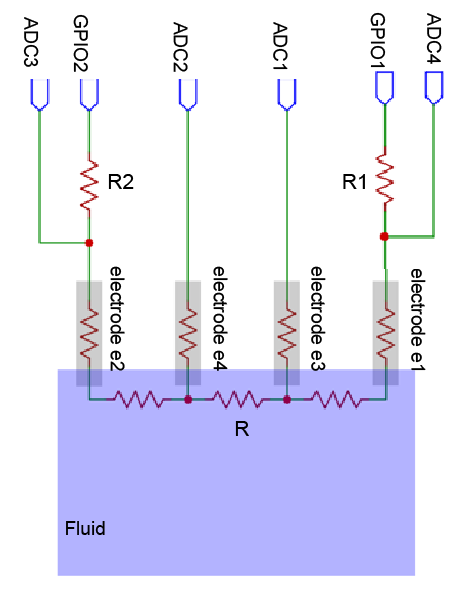
\includegraphics[height=5cm]{Images/4pole_circuit.png}
		\caption[Four-pole EC cell]{Schematic for a four-pole electrical conductivity celll. This circuit can also be driven with an alternating current if the state of electrodes 1 and 2 are alternatingly set to 3.3V and 0V, respectively, in rapid succession. This changes the direction of current flow, minimizing the possible impact of polarization within the fluid and somewhat reducing the tendency of the electrodes to corrode.}
		\labfig{4pole}
	\end{center}
\end{marginfigure}

\paragraph{2-pole vs. 4-pole measurements} Unfortunately, simple 2-pole \texttt{EC} probes based on a single voltage divider only work well for relatively low \texttt{EC}. For this reason, 4-pole electrodes (or other non-contact approaches that are not the subject of this chapter) are typically required for most oceanographic measurements. Furthermore, when 2-pole electrodes are deployed for an extended period of time, corrosion or fouling of the electrodes can significantly change the apparent resistance $R$ between electrodes, completely invalidating the measurements. These problems can be addressed by adding two additional electrodes inside the outer two charged electrodes (\reffig{4pole}). The voltage drop between these two inner (uncharged) electrodes can still be measured by an \adc, but now, because a relatively small fraction of the overall current will flow through the two inner electrodes, the voltage drop between the electrodes and the surrounding fluid will not be particularly large, even if fouling occurs. The voltage drop measured between the inner electrodes divided by the current flowing between the two outer electrodes should still be closely related to the overall resistance $R$ (recall the form of Ohm's law that says $R = V/I$). While $V$ across the inner electrodes isn't precisely equal to $V$ across the outer electrodes, it should still be closely (and linearly) related, so it can still be used as an input for a calibration procedure.  

\paragraph{AC vs. DC measurements} Another major challenge in measuring \texttt{EC} in water using \emph{direct current} (DC) is that water polarizes when a voltage is applied. Water molecules can then reorient themselves, changing the electrical properties of the fluid. This is particularly problematic when a significant amount of current flows, as when the \texttt{EC} is high. The problem can be overcome to some extent by using an \emph{alternating current} (AC)-based method, that is, by switching the direction of current flow at regular (rapid) intervals.  Commercial sensors often use relatively complicated circuitry to create and read the AC current, but we can emulate this relatively easily with a microcontroller simply by switching the states of the positive and negative outer electrodes (i.e., at \texttt{gpio1} and \texttt{gpio2}) at regular intervals.

In the circuit shown in \reffig{4pole}, overall current $I$ can be estimated by measuring the voltage drop across either resistor R1 or R2 by simply recording the \adc measurement associated with that resistor when the adjacent \texttt{gpio} pin is set to \texttt{0V}.  Ohm's law says that $I = V/R$ in that situation. The estimate for $R$ within the fluid can then be made by dividing the voltage difference betwen \adc1 and \adc2 by $I$.  

\subsection{Electrical conductivity circuit assembly.}

A circuit like the one illustrated in \reffig{4pole} can be created simply by laying out the circuit on a breadboard and using the loose ends of several jumper pins as the electrodes\sidenote[][*-10]{
	\begin{kaobox}[backgroundcolor=\SNcolor,frametitlebackgroundcolor=\SNcolor,frametitle=Which microcontroller works with this activity?]\textbf{Full compatibility: \texttt{ESP32} and \texttt{ESP32-S2}.} Because only \texttt{ESP32} and \texttt{ESP32-S2} include the five \adc s required for this activity, they are the only boards that can be used for the complete four-pole electrical conductivity circuit. The pin assignments in the code are for the \texttt{ESP32-S2} and must be changed for use with an \texttt{ESP32}.\\  
\textbf{Parital compatibility: \texttt{ESP8266}.} Despite the fact that it only has one \adc, it is possible to use an \texttt{ESP8266} to record current across either resistor R1 or R2, thereby still performing a two-pole based mesurement.  
	\end{kaobox}
}. The value to use for resistors R1 and R2 depends on the \texttt{EC} of the fluid anticipated as well as on the cell constant of the elecrodes (something that is unlikely to be known in advance).  A value of 250 \si{\ohm} for both resistors is a good starting point. IMPORTANT:  If an \texttt{ESP8266} is to be used, the value of the resistor NOT connected to the \adc should be approximately 3 times the value of the the other resistor to ensure that the limits on the maximum voltage for the \adc are not exceeded.

\begin{marginfigure}[-3cm]
	\begin{center}
		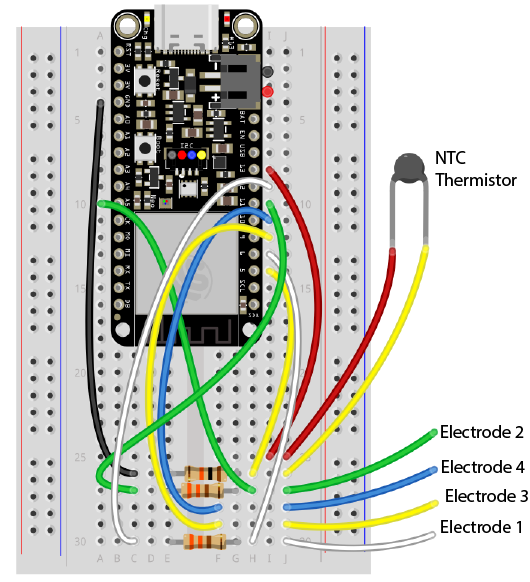
\includegraphics[height=7cm]{Images/ec_breadboard.png}
		\caption[Breadboard layout for four-pole \texttt{EC} cell]{Breadboard layout for four-pole electrical conductivity celll. The four \texttt{EC} electrodes should be connected to four \adc pins, and if the NTC thermistor is used, a $V_{data}$ signal can be connected to a fifth \adc.  The \adc pins can be changed in software.}
		\labfig{fig:ec_breadboard}
	\end{center}
\end{marginfigure}

A breadboard layout illustrating the circuit is provided in \reffig{fig:ec_breadboard}. The layout includes an optional NTC thermistor that can be used for making temperature measurements.

While it is possible to use bare wire for the electrodes, a more robust solution is to use graphite, which will not corrode even in harsh, highly-saline environments. A low-cost source for graphite material is 2-mm diameter pencil lead, available in any art-supply shop. While it is not possible to solder or crimp wire directly to the pencil lead, wire can be wrapped around the lead and then secured in place with shrink tubing.

\begin{marginfigure}[6cm]
	\begin{center}
		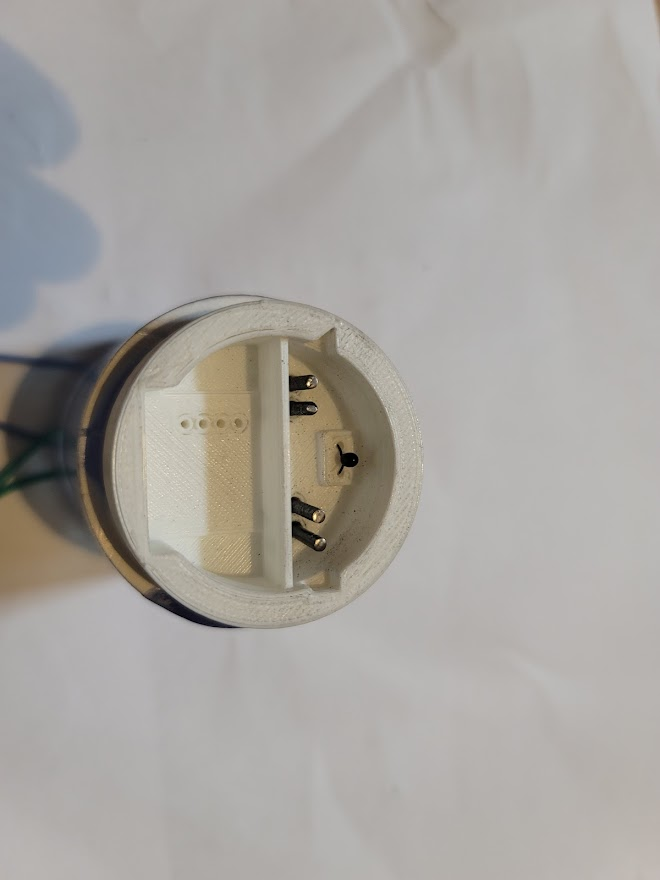
\includegraphics[height=9cm]{Images/AppendixB_cap}
		\caption[3-D printed \texttt{EC cell} housing]{3D printed \texttt{EC} cell housing. A similar housing can be cut from acrylic on a laser cutter. The housing includes mounting holes for electrodes that ensures their geometry can be laid out in a repeatable way. There are also mounting holes for an optional NTC thermistor. The electrodes and thermistor are already mounted in this image.}
		\labfig{fig:3Dcap}
	\end{center}
\end{marginfigure}

The probe is not particularly useful unless it can be immersed in fluid. Obviously, this cannot be done if the bare wires leading up the the electrodes are exposed. Templates for laying out the electrodes can be 3-D printed or laser-cut.  The 3-D printed template is shown in \reffig{fig:3Dcap}. Once electrodes are placed through the mounting holes, they can be fixed in place using hot-melt glue. Glue can then carefully be placed around the outside of the electrodes and over the thermistor to provide a waterproof surface.

\subsubsection{Operation of \texttt{EC} cell}

Once the circuit is laid out, the cell can be run using the following code. The sampling resistor values, maximum \adc counts, and possibly pin assignments should be changed to be consistent with your setup.

\begin{lstlisting}[language=Python]
import machine
from machine import Pin, ADC
import time
import math
import array as arr

#sampling parameters
n = 12 #number of samples per measurement
cycle_time = 100
[on1,off1,on2,off2] = [cycle_time,cycle_time,cycle_time,cycle_time] #sleep time in microseconds
printflag = 0  #flag for extra output

#resistor values 
con_resistance = 272 #resistor (ohms) on either end of conductivity cell
therm_resistance = 9880 #resistor (ohms) in line with thermistor

#max ADC count
max_count = 8191 #for ESP32S2 in single read mode
attenuation_code = ADC.ATTN_11DB #ADC attenuation mode--specifies max readable voltage
max_voltage = 2.730 #max readable voltage--should be calibrated for 11DB atten

#define gpio pins
gpio1 = Pin(11, Pin.OUT)  #connects to P1 through con_resistance
adc1 = ADC(Pin(10))  #connects directly to P4
adc2 = ADC(Pin(9)) #connects directly to P3
gpio2 = Pin(12, Pin.OUT) #connects to P2 through con_resistance
therm_power = Pin(13, Pin.OUT) #connects to either pole of NTC thermistor
adc3_current = ADC(Pin(8)) #Pin A5 on Feather ESP32-S2 -- connects directly to P2
adc4_current = ADC(Pin(6)) #connects directly to P1
adc_therm = ADC(Pin(5)) #connects to either pole of NTC thermistor

\end{lstlisting}

Once pins are assigned and parameters set, the program operates by first setting the maximum \adc voltage as high as possible using the \texttt{ESP32}'s attenuation command.  This should set the maximum voltage to around 2.5 volts, althought this should have been checked earlier for your device.

The code pre-allocates storage arrays before doing any readings in order to quickly store data, thereby allowing the fastest possible AC signal. It then enters the loop where \adc measurements are made. The loop includes short sleep statements to ensure the \adc has time to reset after a reading is made. Once readings are made with the outer \texttt{gpio} pins in one state, the states are switched (so the \texttt{gpio} pin that had previously been set to \texttt{0V} is set to \texttt{3.3V}, and vice-versa. \adc readings are then taken at this polarity state for each \adc pin. When the loop ends, the time taken for executing the loop is used to compute the freqency of the AC signal.

\begin{lstlisting}[language=Python]

#set attenuation so that maximum voltage is at highest possible level
adc1.atten(ADC.ATTN_11DB)
adc2.atten(ADC.ATTN_11DB)
adc3_current.atten(ADC.ATTN_11DB)
adc4_current.atten(ADC.ATTN_11DB)
adc_therm.atten(ADC.ATTN_11DB)

#pre-allocate arrays that will store counts
imeas1 = arr.array('l',[0]*n)
imeas2 = arr.array('l',[0]*n)
p3meas1 = arr.array('l',[0]*n)
p3meas2 = arr.array('l',[0]*n)
p4meas1 = arr.array('l',[0]*n)
p4meas2 = arr.array('l',[0]*n)

starttime = time.ticks_us()
for i in range(n):
    #normal polarity
    gpio1.value(1)
    time.sleep_us(on1)
    imeas1[i] = adc4_current.read()
    p3meas1[i] = adc1.read()
    p4meas1[i] = adc2.read()
    gpio1.value(0)
    time.sleep_us(off1)
    
    #switched polarity
    gpio2.value(1)
    time.sleep_us(on2)
    imeas2[i] = adc3_current.read()
    p3meas2[i] = adc1.read()
    p4meas2[i] = adc2.read()
    gpio2.value(0)
    time.sleep_us(off2)
 
endtime = time.ticks_us()
elapsed_time = endtime - starttime
meas_freq = n/(elapsed_time/1000000)

\end{lstlisting}

Now that data are collected, the code processes the data by computing the relevant currents, voltages, and resistances for the two polarity states (state 1: \texttt{gpio1} high and \texttt{gpio2} low; state 2: \texttt{gpio1} low and \texttt{gpio2} high). It then tosses out the upper and lower quartile and computes the mean of the remaining data to provide a single estimate for I, R, and V for each polarity state.  

\begin{lstlisting}[language=Python]
#pre-allocate arrays for current, voltage drop across poles, and resistance, for flow each direction
i1 = arr.array('f',[0]*n)
i2 = arr.array('f',[0]*n)
V1 = arr.array('f',[0]*n)
V2 = arr.array('f',[0]*n)
R1 = arr.array('f',[0]*n)
R2 = arr.array('f',[0]*n)

#compute current, voltage, and resistance for each sample (do outside sampling loop to maintain sampling timing)
for i in range(n):
    try:
        i1[i] = imeas1[i] / max_count * max_voltage / con_resistance 
        i2[i] = imeas2[i] / max_count * max_voltage / con_resistance 
        V1[i] = (p3meas1[i] - p4meas1[i])/max_count * max_voltage
        V2[i] = (p4meas2[i] - p3meas2[i])/max_count * max_voltage
        R1[i] = V1[i]/i1[i]
        R2[i] = V2[i]/i2[i]
    except:
        R1[i] = -999999
        R2[i] = -999999
        print('Error in resistance computation')

#clean data by sampling middle two quartiles       
upper_index = math.ceil(3*n/4)
lower_index = math.floor(n/4)
sampled_length = (upper_index - lower_index)
resistance1 = sum(sorted(R1)[lower_index:upper_index])/sampled_length
resistance2 = sum(sorted(R2)[lower_index:upper_index])/sampled_length
resistance_average = (resistance1+resistance2)/2
current1 = sum(sorted(i1)[lower_index:upper_index])/sampled_length
current2 = sum(sorted(i2)[lower_index:upper_index])/sampled_length
current_average = (current1+current2)/2

\end{lstlisting}

If the thermistor has been included in the circuit, it can be read here.  Steinhart-Hart coefficients associated with a particular NTC thermistor (by manufacturer \texttt{littlefuse}) are included here, but they can be changed to match what you got by calibration.

\begin{lstlisting}[language=Python]

#read thermistor
A = 0.001125308852122
B = 0.000234711863267
C = 0.000000085663516
therm_count = arr.array('f',[0]*n)
therm_power.value(1)
for i in range(n):
    therm_count[i] = adc_therm.read()
therm_power.value(0)
therm_count_av = sum(sorted(therm_count)[lower_index:upper_index])/sampled_length    
therm_voltage = therm_count_av / max_count * max_voltage
therm_i = therm_voltage / therm_resistance
R_t = (3.3 - therm_voltage)/therm_i
T = 1/((A+B*(math.log(R_t)))+C*((math.log(R_t))**3))-273.15

\end{lstlisting}

Finally, data are processed and printed to the screen. In order to ensure that the sensor was not sampling beyond the range of $V_{max}$ of any of the \adc s that were used in circuit, the maximum and mimimum \adc counts are also computed and printed out.  If the maximum is at the value of the maximum count, the reading is suspect.

\begin{lstlisting}[language=Python]

    
#find maximum and minimum counts to see if out of range of ADC:
arrays_of_counts = [imeas1, imeas2, p3meas1, p3meas2, p4meas1, p4meas2]
oldmax = 0
oldmin = max_count
for array in arrays_of_counts:
    maximum = max(max(array),oldmax)
    minimum = min(min(array),oldmin)
    oldmax = maximum
    oldmin = minimum

#Print output
if printflag:
    for i in range (n):
        print(f"R1 = {R1[i]:.2f}, R2 = {R2[i]:.2f}, V1 = {V1[i]:.2f}, V2 = {V2[i]:.2f}, i1 = {i1[i]:.2f}, i2 = {i2[i]:.2f}")
        print(f"adc_count3 = {imeas2[i]}, adc_count4 = {imeas1[i]}, adc1_1 = {p3meas1[i]}, acd1_2 = {p4meas1[i]}, adc2_1 = {p4meas1[i]}, adc2_2 = {p4meas2[i]}")
outputstring = f"R1 = {resistance1:.2f}, R2 = {resistance2:.2f}, R_av = {resistance_average:.2f}, "
outputstring += f"i1 = {current1:.5f}, i2 = {current2:.5f}, i_av = {current_average:.5f}, "
outputstring += f"T = {T:.2f}, freq = {meas_freq:.1f} hz, max_count = {maximum}, min_count = {minimum}"
print(outputstring)
    
\end{lstlisting}

\loadMilestone{mlst:04i} % load milestone with tags id: mlst:04i

\subsection{Electrical conductivity circuit calibration}

It is impossible to completely controll all the variables that might affect the output of an analog sensor. In the case of the electrical conductivity cell, these variables include things like the exact length and angle of the exposed electrodes, the exact value of the resistors included in the circuit, the length of wire leading up to the electrodes (this wire has some resistance), the voltage reference used by the microcontroller's \adc, any fouling/corrosion of the electrodes, and so on.  Because we cannot know these parameters, the only way to make our sensor useable is to empirically search for a relationship between the physical parameter of interest and what we can read from the sensor.

The first step in such a calibration normally involves identifying a calibration standard. In the case of \texttt{EC} cells, this is often handled by mixing up a solution of an electrolyte for which the relationship between \texttt{EC} and concentration is well known. The quality of the calibration will never be higher than the precision to which the \texttt{EC} of the calibration standard is known, so care must be taken to ensure that the standard is of high quality. The National Institute of Standards in Technology (NIST) provides guidelines for the production of high-quality standards, which are referred to as \emph{NIST-traceable}.  Alternatively, a highly precise, well calibrated laboratory instrument can be used to measure the \texttt{EC} of a calibration solution mixed in the lab.  

\begin{kaobox}[frametitle=Mixing up an \texttt{EC} calibration fluid]
Potassium Chloride (KCl) is often used as a calibration standard for \texttt{EC} cells. A 0.1 molar solution has a specific conductance $\kappa_s$ of approximately \num{1.3e4} \si{\micro\siemens\cm}. For KCl, this concentration is equivalent to 7.43 g KCl/L water.
\end{kaobox}

\subsubsection{Typical calibration procedure}
Calibration of an \texttt{EC} device typically involves tabulating the output from the device across the range of conductivites of interest. It is good practice to perform more than one measurement at a given \texttt{EC}. For instance, a calibration based on measurements made in tripilicate would involve making three sensor readings for each known \texttt{EC} value. Having multiple measurements for a single \texttt{EC} improves the ability to identify where the sensor output becomes unreliable.

Once data are collected, analysis must be performed to develop the empirical relationship between sensor reading and \texttt{EC}. A number of analytical approaches are available for this task, and many of these are beyond the scope of this textbook. We briefly touch on three simple approaches here\sidenote[][*]{
		\begin{kaobox}[backgroundcolor=\SNcolor,frametitlebackgroundcolor=\SNcolor,frametitle=Computational Links]Each of the three approaches described in this section are illustrated in a Jupyter Notebook that you can use for your own computations.  The notebook is available at \htmladdnormallink{\texttt{Calibration Examples}}{https://github.com/jwlauer/EnvironmentalSensing/tree/master/AnalysisCode/Calibration}
		\end{kaobox}
	}
: 1) direct computation of the mean cell constant, 2) linear regression, which produces a simple linear relationship between $\frac{1}{R}$ and \texttt{EC}, and 3) log-log regression, which ultimately results in a power function relationship of the form 

\begin{equation}\label{eq:ec_power}
	\frac{1}{R}=a\kappa ^b.  
\end{equation}

\subsubsection{Direct computation of cell constant}
In the first approach, we assume that Equation \ref{eq:cell_const} describes the functional relationship precisely, and that the cell constant does not depend on \texttt{EC}.  Under these assumptions, we can use each reading to independently compute $k$

\begin{equation}\label{eq:cell_i}
	k_i=\kappa _i R_i  
\end{equation}

where the subscipt $i$ denotes the value associated with the ${i_{th}}$ data pair.  The cell constants can then be averaged to find an overall estimate. 

\begin{equation}\label{eq:ave_cell_const}
	\overline{k} = \frac{\sum\limits_{i=1}^n k_i}{n}
\end{equation}

Confidence limits $CL$ on the estimated mean cell constant can be computed using a statistical t-test. 

\begin{equation}\label{eq:ec_power}
	CL = \overline{k} \pm t_{({1-\alpha/2,n-1})}\frac{s}{\sqrt{n}}
\end{equation}

where $t$ is the value of the $t$ statistic at significance level $\alpha$ and $n-1$ degrees of freedom ($n$ is normally the number of samples) and $s$ is the sample standard deviation. Note that $s/\sqrt{n}$ is often referred to as the \emph{standard error}.  Keep in mind that these confidence limits characterize the precision of our estimate for $\overline{k}$, not the confidence we will have in any single measurement we later make using our device.
 
\subsubsection{Calibration by simple linear regression}

Imperfections in our \texttt{EC} circuit design (and particularly the presence of internal resistance within each electrode) means that we don't necessary expect Equation \ref{eq:cell_const} to hold across the entire range of \texttt{EC}. We can account for this to some exent by including an offset (or y-intercept) in the relationship between $\frac{1}{R}$ and $\kappa$.

\begin{equation}\label{eq:linear_calibration}
	\frac{1}{R}=b_1\kappa +b_0.  
\end{equation}

where $b_1$ is the slope of the linear relationship and $b_0$ is the y-intercept. Essentially all statics packages include the ability to perform linear regression, so computing the slope and intercept from the observed $\frac{1}{R}$ and $\kappa$ is straighforward. However, we also wish to characterize the confidence we have in the \texttt{EC} estimate we make from this relationship at a given sensor reading. Several methods for providing these limits are available.  Here, we summarize a method presented in \cite{LAVAGNINI} for adding a \emph{confidence intervals} to a calibration equation developed by linear regression.

For generality, we use the variable $y_i$ to represent a sensor reading and the variable $x_i$ to represent the corresponding physical value.  In the case of the \texttt{EC} sensor, 
\begin{equation}
	y_i = \frac{1}{R_i}  
\end{equation}

and
\begin{equation}
	x_i = \kappa_i.  
\end{equation}


In practice, after calibration is complete and the user wishes to use the calibrated instrument to collect data, the value of the physical parameter of interest (e.g., \texttt{EC}) will be computed based on the mean of one or more sensor readings. The estimate of the physical parameter computed from the mean of $m$ sensor readings $\tilde{y}_m$ is denoted by $\tilde{x}_0$, and its variance $s_{\tilde{x}_0}^{2}$ is given by \cite{LAVAGNINI} as: 

\begin{equation}\label{eq:var_readings}
	s_{\tilde{x}_0}^{2}=\frac{s_{y/x}^{2}}{b_{1}^{2}}\left (\frac{1}{m}+\frac{1}{n}+\frac{(\tilde{x}_0-\overline{x})^2}{\sum\limits_{i=1}^n \left ( x_i-\overline{x} \right )^2} \right )
\end{equation}

where $\overline{x}$ is the mean of the observed physical parameter in the calibration dataset (e.g., the mean of all \texttt{EC}s values used as part of the calibration process),  

\begin{equation}\label{eq:regression_var}
	s_{y/x}^{2}=\frac{\sum\limits_{i=1}^n \left ( y_i-\tilde{y}_i \right )}{n-2},
\end{equation}

and $\tilde{y}_i$ is the value of the sensor output (e.g., $\frac{1}{R_i}$) that would be estimated from the regression equation at $x_i$,

\begin{equation}\label{eq:linear}
	\tilde{y}_i=b_1 x_i +b_0.  
\end{equation}

The statistic $s_{y/x}^2$ is referred to as the residual variance of the regression. 

This can be used to develop a confidence interval on the corresponding physical parameter $\tilde{x}_0$, 

\begin{equation}\label{eq:confidence}
	\hat{x}_0^\pm = \tilde{x}_0 \pm t_{({1-\alpha/2,n-2})}s_{\tilde{x}_0}
\end{equation}

where $\hat{x}_0^\pm$ represents the upper and lower limits on $\tilde{x}_0$.  In this case, we would expect there to be a $1-\alpha$ chance that an our estimate $\tilde{x}_0$ falls within these limits.

\begin{marginfigure}[0cm]
	\begin{center}
		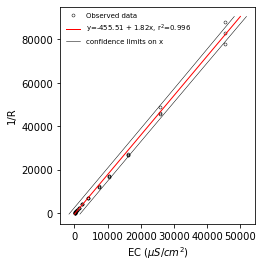
\includegraphics[height=9cm]{Images/linear_confidence.png}
		\caption[Confidence Limits on Linear Regression]{Confidence limits on the linear regression of raw \texttt{EC }calibration data.}
		\labfig{fig:linear_confidence}
	\end{center}
\end{marginfigure}

An example of a linear regression calibration curve is given in figure \reffig{fig:linear_confidence}. The points from which the curve was generated were collected in triplicate at each \texttt{EC} value.  Data points are not evenly spaced because they were produced by diluting the previous calibration fluid by a specified amount.  This makes the regression particularly sensitive to the measurements made at the highest \texttt{EC} value. This sensitivity can be addressed to some extent by performing the regression on log-transformed data, as described in the next section.

\subsubsection{Calibration by log-log regression}

When data span several orders of magnitude, it is often more appropriate to perform a regression on the natural logarithms of data than on the data themselves. This can be accomplished by simply repeating the procedure outlined in the previous section with the natural logarithms of the data as input

\begin{equation}
	y_i = ln\left ( \frac{1}{R_i} \right )
\end{equation}

and
\begin{equation}
	x_i = ln(\kappa_i).  
\end{equation}

\begin{marginfigure}[0cm]
	\begin{center}
		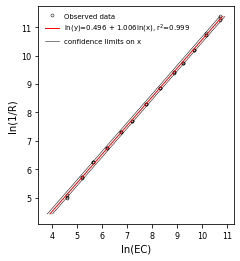
\includegraphics[height=9cm]{Images/log_confidence.png}
		\caption[Confidence Limits on Log-Log Regression]{Confidence limits on the log-log regression of \texttt{EC }calibration data.}
		\labfig{fig:log_confidence}
	\end{center}
\end{marginfigure}

The rest of the procedure is the same as before.  This produces regression line and confidence limits describing the logs of the data, as illustrated in \reffig{fig:log_confidence}, which was produced using the same data as was used in \reffig{fig:linear_confidence}. Notice that the points now appear much more evenly spaced. This is because a given \texttt{EC} in the calibration standards were roughly a constant fraction of the \texttt{EC} of the next higher \texttt{EC} standard.

Once the regression line and confidence limits are known on the log scale, they can be re-transformed to the linear scale by taking antilogs (in this case, using the exponential function). 

\begin{equation}
	e^{ln(y)} = e^{b_1 ln(x) + b_0}
\end{equation}

This results in a final regression equation of power-function form,

\begin{equation}
	y = b_0 x^{b_1}
\end{equation}

or, for the case of the \texttt{EC}-based calibration data presented here,

\begin{equation}\label{power_calibration}
	\frac{1}{R} = b_0 \kappa^{b_1}
\end{equation}

For practical computations, the inverse of Equation \ref{power_calibration} would be used to compute \texttt{EC} from a given sensor value.

\begin{equation}\label{power_calibration}
	\kappa = {b_0}^{-\frac{1}{b_1}}\left ( \frac{1}{R}\right )^{\frac{1}{b_1}} 
\end{equation}

\begin{marginfigure}[0cm]
	\begin{center}
		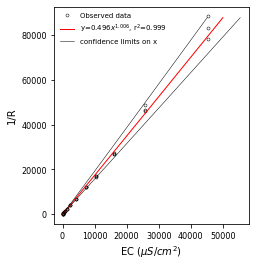
\includegraphics[height=9cm]{Images/log_confidence_retransformed.png}
		\caption[Confidence Limits on Retransformed Log-Log Regression]{Confidence limits on the log-log regression of \texttt{EC }calibration data after retransformation to a linear scale.}
		\labfig{fig:log_confidence_retransformed}
	\end{center}
\end{marginfigure}

Once transformed back to the regular linear scale, as in Figure \reffig{fig:log_confidence_retransformed}, it becomes clear that the confidence intervals do a much better job bounding the calibration data than do the limits associated with the simple linear regression presented in Figure \reffig{fig:linear_confidence}.

\loadMilestone{mlst:04j} % load milestone with tags id: mlst:04j






\newpage


\section{Environmental sensing with time: measuring light intensity with frequency}
\labsec{light_freq}
Light is a key variable in the physics, chemistry and biology of most terrestrial and marine environments.
Light is an interesting and complex environmental characteristic in part because of its variable effects across the UV, visible and IR ranges of the electromagnetic spectrum, and because its intensity varies many orders of magnitude over short time and space scales.
These properties also make light a challenge to measure.

Sensors are widely available that respond to light by varying resistance, analogous to thermistors' responses to temperature.
An example is a \htmladdnormallink{photoresistor}{https://en.wikipedia.org/wiki/Photoresistor}.
We could therefore measure light with a voltage divider incorporating a photoresistor, using a very similar approach to calibration and implementation as for the thermistor voltage divider.

In this section, we will instead use an analog sensor that signals light levels using time --- specifically, the frequency of electrical pulses --- rather than voltage.
Your \texttt{ESP8266}, like many microcontrollers, can measure time intervals with relatively high resolution over a much larger range of magnitudes than its \adc can measure voltage.
As you might expect, this broad measurement range means that time-based sensors enable the \texttt{ESP8266} to quantify light with similarly higher resolution and larger intensity range, compared to voltage-based sensors.

To compound this advantage, it is very easy (using components designed for the purpose) to ``\emph{divide}'' a frequency signal -- that is, to reduce its frequency by a standard factor of 8 or 10.
If a sensor frequency approaches the upper limits of a microcontroller's measurement capabilities, dividing the signal in this way provides a reduced frequency that is within the microcontroller's limits.
It is then easy to convert the reduced frequency back to the original, with multiplication by the same factor.

To take advantage of this increase in sensor range, the circuit you will build will have two sub-circuits: One measures frequency directly from the light sensor.
The other measures the reduced frequency output from a divider.
As part of the sensor design, you will determine a suitable criterion for choosing which sub-circuit's measurements are most accurate at different light levels.

\subsection{Measuring light with frequency}
The sensor you will use in this circuit is the \htmladdnormallink{TSL237 High-Sensitivity Light-to-Frequency Converter}{https://ams.com/documents/20143/36005/TSL237\_DS000156\_3-00.pdf/4aa35672-5c5e-3bb7-4d6b-92f4c76a3531}.
Like most of the analog sensors we've considered, this sensor has three wires.
Two are the usual inputs, $GND$ and $V_{in}$.
The third is the output, $V_{data}$, which oscillates between $GND$ and $V_{in}$ at a frequency, $f$, proportional to light intensity.

Important information about this sensor is contained in the \texttt{datasheet} linked above.
The oscillation frequency in absolute darkness, $f_{dark}$, is typically around \texttt{0.1 Hz} (it varies somewhat with temperature).
The ``\texttt{full-scale frequency}'' --- the highest frequency that can be put out by the sensor --- is $f_{full}=1000kHz=1MHz$.
Figure 9 in the datasheet shows how irradiance, $E$, varies with frequency across more than 5 orders of magnitude in both quantities.

The responsiveness of the \texttt{TSL237} sensor varies with wavelength of the incident light, at maximum near 700nm and dropping to half the maximum at approximately 400nm and 875nm (Figure 10 of the datasheet).
Figures 13 and 14 show how responsiveness varies with the angle of the incident light --- it has relatively high responsiveness ($>75\%$) within roughly $30^\circ$ of the sensor's centerline.

Both color and angular variation (which are present for nearly all light sensors) often introduce some complications in interpretation of light intensity data in a specific location.
For example, across depth in an ocean or lake, the ambient light usually becomes bluer, as redder light is more quickly absorbed.
Depending on scattering by particles, the angular distribution of light rays may also broaden substantially.
Under a forest canopy, much of the ambient light might be in the green part of the spectrum, which is not absorbed by photosynthesizing plants.
In environments like these, informative metrics of light intensity may require separate measurements in different parts of the color spectrum and at different angles.

With all these caveats in mind, we can see from the datasheet that the irradiance responsivity of the \texttt{TSL237} sensor is $R_e=2.3 \frac{\mathtt{kHz}}{\mathtt{uW}/\mathtt{cm}^2}$.
This implies that a \emph{nominal irradiance} --- subject to corrections for wavelength, angle and temperature --- is given by
\begin{equation}\label{irrad}
E_e = \frac{1}{R_e} (f-f_{dark}) .
\end{equation}
Notice that, in Equation \ref{irrad}, the calculation for $R_e$ assumes frequency in units of \texttt{kHz}.
Because we typically use \htmladdnormallink{SI units}{https://en.wikipedia.org/wiki/International_System_of_Units}, we need to remember to convert from \texttt{Hz} to \texttt{kHz} when we apply this formula.

Equation \ref{irrad} gives us an approximate way to calibrate irradiation as a function of frequency, and to predict frequency for specific irradiances.
This calibration is ``approximate'' because it neglects variation between individual sensors.
It also neglects adjustments for the color and angle of incident light.

Because $f_{dark}$ is very small compared to $f$ in all situations except nearly absolute darkness, and because the errors associated with wavelength, angle and temperature are typically much larger, we can usually neglect the $f_{dark}$ term in Equation \ref{irrad}.
In that case we can simplify to a proportionality,
\begin{equation}\label{irrad2}
E_e \approx \frac{1}{R_e} f,
\end{equation}
where again $f$ is measured in \texttt{kHz}.

\subsubsection{\howto Assemble and test a frequency-based light sensor circuit}
\labsec{tsl237}
\begin{marginfigure}[-4cm]
	\begin{center}
		\htmladdnormallink{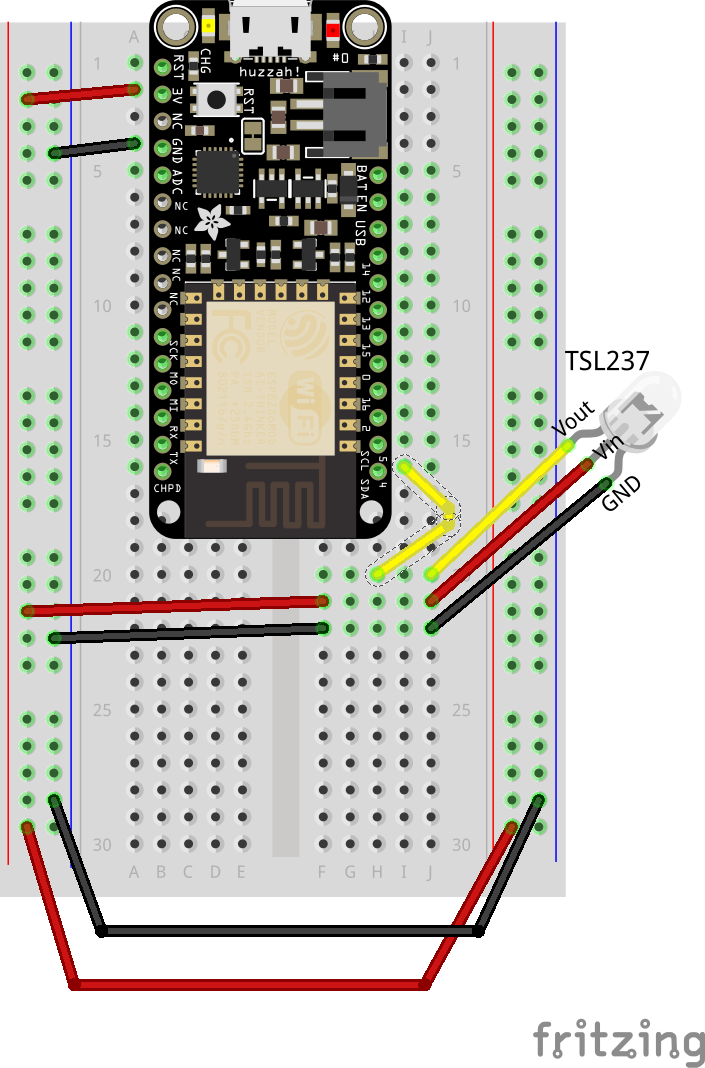
\includegraphics[width=\MFW]{Fritzing/feather_tsl237module1_bb.png}}{https://publicsensors.org/IntroSensors/Fritzing/feather_tsl237module1_bb.png}
		\caption[Light sensor sub-circuit 1 schematic]{An illustration of the circuit layout for sensing light using a \texttt{TSL237} Light-to-Frequency sensor.
		This schematic represents sub-circuit 1, in which frequency is read directly from the sensor.
		The sensor, labeled \texttt{TSL237}, is represented by an image of an \texttt{LED}, because no image of the \texttt{TSL237} is currently available in the Fritzing software.
		The 8 bottom rows on the breadboard are left open to leave room for sub-circuit 2.
		Red wires represent \texttt{3.3 volts}, black wires represent \texttt{GND}, and yellow wires represent the frequency-modulated sensor output.}
		\labfig{feather_tsl237module1}
	\end{center}
\end{marginfigure}
An example layout of the \texttt{TSL237} sub-circuit is shown in \reffig{feather_tsl237module1}.



\begin{enumerate}
	\item \textbf{Starting with the \texttt{ESP8266} and power/ground rails in their usual configurations, connect the \texttt{Vin} and \texttt{GND} pins to their respective rails.}

	The pin assignments for the \texttt{TSL237} are shown in Figure 3 of the datasheet.
	With the sensor facing upwards (the little plastic focusing hemisphere pointing up) and wires pointing towards you, \texttt{GND} is the left wire, \texttt{Vin} is the middle wire, and \texttt{Vout} is the right wire.

	\smallskip
	In the schematic, we've illustrated jumpers between the sensor and the breadboard.
	These are to make clear how the inputs and output are connected.
	These jumpers are optional --- you may connect the sensor directly into the breadboard, or use female-male jumpers between the sensor and the breadboard.

%	\smallskip
%	Very long wires between the sensor and the microcontroller can affect the sensor reading.
%	So, it's best to restrict these wires to about the length of standard jumpers.

	\item \textbf{Connect the sensor's \texttt{Vout} to \texttt{Pin 4} on the microcontroller.}

\end{enumerate}
The hardware for sub-circuit 1 is now complete.

\smallskip
To measure frequency from the \texttt{TSL237} sensor, we will first measure its \texttt{\textbf{period}}.
The period is the time taken for a complete high/low cycle of the oscillating voltage on \texttt{Pin p}.
The \texttt{TSL237}'s frequency is the inverse of this period.

To measure the period, we will use a modification of code posted on the \htmladdnormallink{MicroPython forum}{https://forum.micropython.org/viewtopic.php?f=18\&t=5724\&p=32921}:
\lstinputlisting[language=Python,label=FrequencyMedian,caption={\htmladdnormallink{\texttt{period\textunderscore median.py}}{https://github.com/publicsensors/IntroSensors/blob/main/Codes/period_median.py}: A Python function to calculate the period of an oscillating voltage.}]{Codes/period_median.py}
This code uses a \Micropython  utility called \lstinline{time_pulse_us} to measure the period, in microseconds, of the  oscillating voltage on \texttt{Pin p}.

To improve precision, the code repeats this measurement \texttt{n} times, and returns the median value.
It also returns \texttt{True} if the measurements completed without errors.
This result is presented as a Python tuple, \lstinline{(per,valid)}, where \lstinline{per} is the measured period in $\mu s$ and \lstinline{valid} is \texttt{True} for a successful measurement.

One thing to know about the \lstinline{time_pulse_us} function is that, if the pin it is monitoring does not change state within the interval \texttt{timeout}, an error is triggered.
In this case, \lstinline{time_pulse_us} returns \texttt{-1} or \texttt{-2} as an error message.
Two things happen if this error occurs.
The \lstinline{median_of_n} code returns \texttt{False} for \lstinline{valid}, flagging the error status.
Also, the  \lstinline{median_of_n} code returns the value of \texttt{timeout} for \lstinline{per}, instead of a measured period.

\emph{That is, the} \lstinline{median_of_n} \emph{code returns the either the measured pulse interval or the parameter} \lstinline{timeout}\emph{, whichever is lower}.
In other words, \texttt{timeout} is the maximum value for the period reported by \lstinline{median_of_n}, even if the true period is longer.
This is something to keep in mind as you assess the sensor measurements.

The code is designed this way for two reasons.
One is to prevent error messages from contaminating frequency estimates from the light sensor.
Spurious measurements of \texttt{-1} or \texttt{-2}, if treated like true measurements, would erroneously reduce the reported period and increase the inferred light intensity.
It could even give negative frequency values!
The other is to prevent the \lstinline{median_of_n} function from being stuck for an indefinite period if there are no pulses.
This could happen if the sensor is accidentally detached or damaged, or takes a reading in near-absolute darkness.


\begin{enumerate}[resume]
	\item \textbf{Copy the \lstinline{period_median.py} file containing the \lstinline{median_of_n} function onto your microcontroller.}
	\item \textbf{Test your light sensor circuit using the commands:}
\begin{lstlisting}[language=Python]
from period_median import median_of_n
from machine import Pin
p4 = Pin(4, Pin.IN)
timeout=300000
nrep=7
median_of_n(p4,nrep,timeout,verbose=True)
\end{lstlisting}
	These commands first import the necessary modules.
	In your circuit, \texttt{Vout} from the \texttt{TSL237} is attached to \texttt{Pin 4}, so this pin is initialized as \texttt{p4} and used in the function call.
	The parameter \texttt{timeout} is here set to \texttt{300000} $\mu s$, or \texttt{0.3 s}.
	The measurement is repeated \texttt{nrep=7} times.
	In this example, \texttt{verbose=True} is used to print out the individual measurements.
	The results will be similar to
\begin{lstlisting}[language=Python]
52 [41, 51, 52, 52, 53, 54, 54]
(52, True)
\end{lstlisting}
	The verbose output gives you a sense for the precision of successive measurements, under essentially constant ambient light conditions.

	\smallskip
	Except when testing, it's often helpful to set \lstinline{verbose=False}, to see only the second line of this output (the median of measured periods, and whether the measurements completed successfully).

	\item \textbf{Take several measurements of period under different light conditions (e.g. shade the sensor with your hand, and shine a bright light directly on it).}

	Enter the measurements of \texttt{TSL237}'s period from \lstinline{median_of_n} in one column of a spreadsheet, under the column header \texttt{Period}.

	\item \textbf{Calculate frequency from your period measurements.}

	In the next column, enter the header \texttt{Hz}.
	Next to each value in the \texttt{Period} column, enter the formula to calculate 1000000/\texttt{Period}.
	Because \lstinline{median_of_n} measures time in microseconds, this quotient is the frequency of the signal in \texttt{herz} (cycles per second, abbreviated \texttt{Hz}).

	\smallskip
	In the next column, enter the header \texttt{kHz}, representing frequency in units of \texttt{kiloherz}.
	Next to each value in \texttt{Hz} column, enter the formula to calculate \texttt{Hz}/1000.
	This column now contains your observed frequencies converted to \texttt{kHz}, which are the units expected for in Equation \ref{irrad}.

	\item \textbf{Critically assess your observations.}

	What is the largest and smallest period and frequency you observe in your tests?
	Do you see any evidence of limits to the range of the \texttt{TSL237}/\texttt{ESP8266} combination, either at high or low light intensities?
\end{enumerate}

\loadMilestone{mlst:04f} % load milestone with tags id: mlst:04f
%A ``driver'' is code designed to interface with a piece of hardware.
%In the case of your light sensor, a driver should be a function that provides a clear and intuitive way to measure light.
%\ref{irrad}

\subsection{Dividing frequency to increase sensor range}
\labsec{divider}
The sub-circuit you set up to measure light in \refsec{tsl237} should work well over a range of light conditions.
However, there are limits to this range.
At very low light levels, readings from the sensor are limited by the parameter \texttt{timeout}, which the longest pulse interval that can be measured by the \lstinline{median_of_n} script.

At very high light levels, readings are limited by the microcontroller hardware.
The \lstinline{time_pulse_us} function cannot accurately measure intervals shorter than a few microseconds.
The \texttt{tsl237} light sensor gives a frequency up to 1 $MHz$.
This corresponds to a 1 $\mu s$ pulse interval, which is much too short for the \texttt{ESP8266} to resolve.

How can we increase the range of light levels over which meaningful measurements can be taken by your \texttt{TSL237}/\texttt{ESP8266} instrument?
One approach is to add an additional sub-circuit to the existing circuit, that implements a counter/divider, called a \htmladdnormallink{CD4017B} {https://www.ti.com/lit/ds/symlink/cd4017b.pdf}.

The \texttt{CD4017B} takes in an input frequency, and outputs a frequency reduced by a factor of 10.
More specifically, it sends pulses to different pins, representing ``counts'' from 0 to 9.
A microcontroller \texttt{GPIO} attached to the \texttt{CD4017B} pin associated with one of those pins will see only every 10th input pulse.
Some periods in \texttt{TSL237} output that are too short for the \texttt{ESP8266} to measure directly can be measured after being ``lengthened'' by  this factor of 10.
As you can see from \ref{irrad2}, this extends the range of your instrument into roughly $10\times$ higher light intensities.

However, there is a tradeoff:
The longest \texttt{TSL237} period that can be measured is also reduced by a factor of 10, meaning that the range of the instrument is reduced at lower light intensities.
Also, its resolution is reduced by this same factor of 10.

Clearly, the ideal would be the best of both worlds --- to use the high resolution, direct measurement of \texttt{TSL237} when it is within the \texttt{ESP8266}'s capabilities, and to use the frequency-divided \texttt{CD4017B} output when light levels are too high for direct measurements.
The activities in this section take you through implementing this improved instrument.
First, you will build a new sub-circuit using a \texttt{CD4017B} to generate a $10\times$-reduced frequency signal.
Then, you will code a driver to automatically select between the direct and reduced frequency signals, to obtain the best light measurement.

%To identify situations in which light levels exceed the capacity of the sub-circuit constructed in \refsec{tsl237}, and to get more accurate readings in those cases, you will now add sub-circuit 2 to your sensor.
%\smallskip
%By measuring the period of signals coming from the \texttt{CD4017B}, sub-circuit 2 effectively extends your microcontroller's time measurement capacity to a ten-fold higher light intensity.

%In effect, the \texttt{CD4017B} shifts the working range of the \texttt{TSL237} to tenfold higher light intensity.
\subsubsection{\howto Measure divided frequency from a light sensor}
\labsec{cd4017b}
\begin{marginfigure}[0cm]
	\begin{center}
		\htmladdnormallink{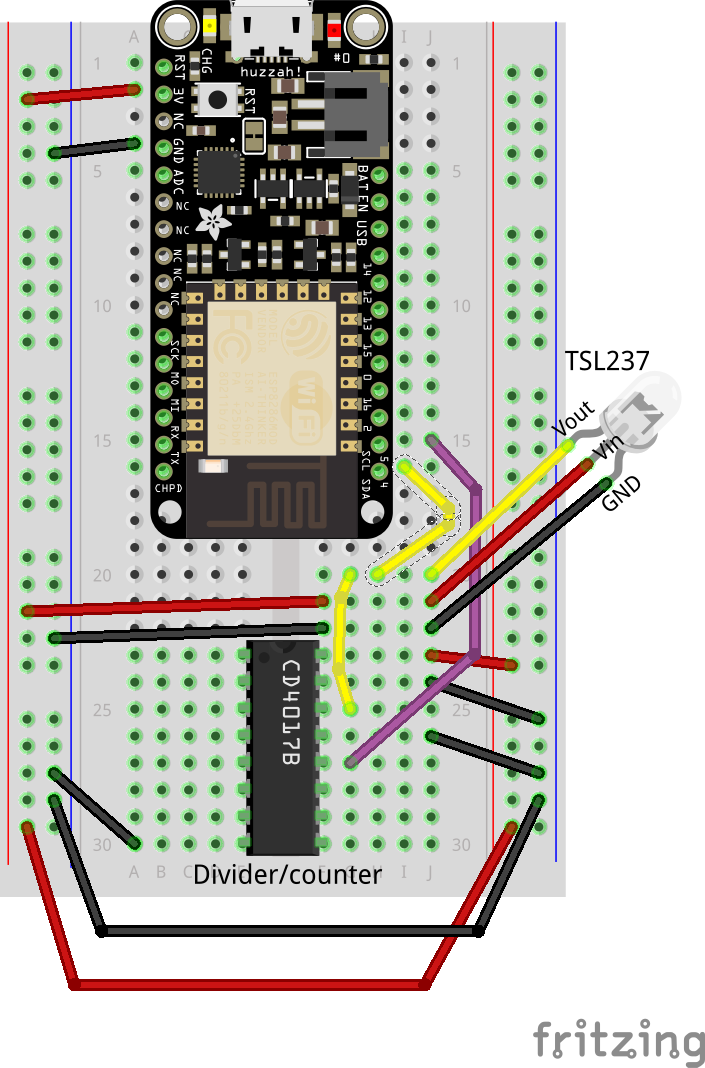
\includegraphics[width=\MFW]{Fritzing/feather_tsl237_bb.png}}{https://publicsensors.org/IntroSensors/Fritzing/feather_tsl237_bb.png}
		\caption[Complete light sensor circuit schematic]{An illustration of the circuit layout for sensing light coupling a \texttt{CD4017B} divider/counter with a \texttt{TSL237} Light-to-Frequency sensor.
		Sub-circuit 2 is an addition to sub-circuit 1, which is not modified.
		Wire colors retain the same meaning as in sub-circuit 1, with the additional purple wire representing divided frequency from the frequency-modulated sensor output.
		in which frequency is read directly from the sensor.}
		\labfig{feather_tsl237}
	\end{center}
\end{marginfigure}
The layout for adding sub-circuit 2 to your sensor assembly is shown in \reffig{feather_tsl237}.

\begin{enumerate}
	\item \textbf{Place your \texttt{CD4017B} on the breadboard.}

	The orientation of the \texttt{CD4017B} is indicated by the semi-circular indentation on one end.
	This is the upper end, which goes closest to the microcontroller.

	\item \textbf{Connect power and ground to the \texttt{CD4017B}.}

	The pins on the \texttt{CD4017B} are explained in the \htmladdnormallink{CD4017B datasheet} {https://www.ti.com/lit/ds/symlink/cd4017b.pdf}.
	The lower left pin is \texttt{GND}.
	The upper right pin is \texttt{Vin}, which in this case is connected via the power rail to \texttt{3.3 volts} from the microcontroller.

	\smallskip
	There are two additional ground connections.
	\begin{itemize}
		\item[$\circ$] \textbf{Connect the \texttt{RESET} pin, immediately below \texttt{Vin}, to \texttt{GND}.}
		\item[$\circ$] \textbf{Connect the \texttt{CLOCK INHIBIT} pin, two rows below the \texttt{RESET} pin, to \texttt{GND}.}
	\end{itemize}
	Both these pins modify the state of the \texttt{CD4017B} in ways that are not needed in our circuit.

	\item \textbf{Connect \texttt{Vout} from the \texttt{TSL237} to the \texttt{CLOCK} pin on the \texttt{CD4017B}.}

	The \texttt{CLOCK} pin is the input frequency signal for the \texttt{CD4017B}.
	Here, we connect it to \texttt{Vout} from the \texttt{TSL237}, which carries the voltage oscillating at the frequency to be divided.

	\item \textbf{Connect the \texttt{CARRY OUT} pin on the \texttt{CD4017B} to \texttt{Pin 5} on your \texttt{ESP8266}.}

	The \texttt{CARRY OUT} pin is the \texttt{CD4017B}'s output, which has $\frac{1}{10}$th the frequency of the \texttt{CLOCK} pin input.

	\item \textbf{Test your frequency dividing circuit using the commands:}
\begin{lstlisting}[language=Python]
from period_median import median_of_n
from machine import Pin
p5 = Pin(5, Pin.IN)
timeout=300000
nrep=7
median_of_n(p5,nrep,timeout,verbose=True)
\end{lstlisting}
	Most of this code is the same as in the sub-circuit 1 test.
	The only change is in pin number, from 4 to 5.
	The results will be something like
\begin{lstlisting}[language=Python]
536 [533, 533, 534, 536, 536, 537, 538]
(536, True)
\end{lstlisting}
	\item \textbf{Repeat the assessment from \refsec{tsl237}, taking several measurements under different light conditions, calculating frequency from period, and critically assessing your observations.}

	What is the largest and smallest period and frequency you observe in the new tests?
	Do you see any evidence of changes in limits to the sensor's range, either at high or low light intensities, when the frequency signal is divided by the \texttt{CD4017B}?

\end{enumerate}
\loadMilestone{mlst:04g} % load milestone with tags id: mlst:04g



\subsection{Optimizing a light sensor driver}
\labsec{opt_driver}
With a working circuit that takes both direct and reduced frequency signals, you are now ready to code a driver to automatically select the best light measurement.

The basic idea is that, for very low light levels, you want to measure period directly from the \texttt{TSL237}.
For very high light levels, you want to measure the frequency divided period from the \texttt{CD4017B}.
At intermediate light levels, it may not matter which way you measure period, because both are acceptably accurate.

How can you determine what is ``high'', ``low'' and ``intermediate'' for your instrument?
One simple approach is to construct a log-log plot, with direct period measurements on the vertical axis and divided period measurements on the horizontal axis.
In such a plot, we expect that within the ``intermediate'' range --- where both methods are accurate --- the measurements will fall on the $1:10$ line.

We also expect that, at very high light levels, the direct measurements will ``bottom-out'' --- that is, they'll reach the smallest measurable interval on the \texttt{ESP8266} --- while the divided measurements continue to decrease.
If so, those points on the plot will lie above the $1:10$ line, and their vertical coordinates will never be below the smallest measurable interval.

Conversely, at very low light levels, the divided measurements will ``top-out'' --- that is, they'll reach the \texttt{timeout} limit --- while the direct measurements continue to increase.
If so, those points on the plot will lie above the $1:10$ line, and their horizontal coordinates will never be above the \texttt{timeout} limit.


\begin{marginfigure}[-8cm]
	\begin{center}
		\htmladdnormallink{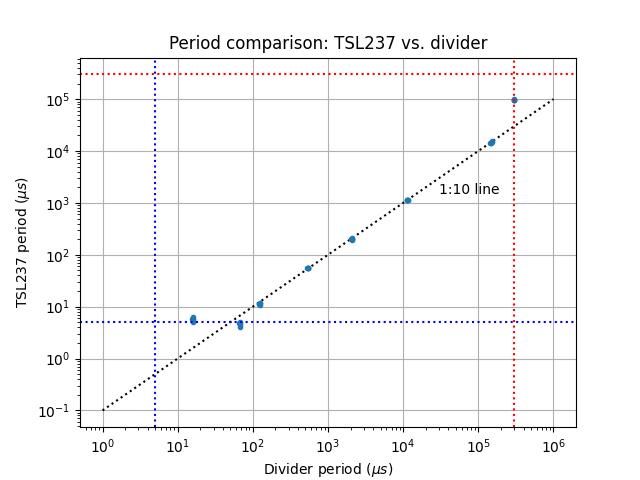
\includegraphics[width=\MFW]{Images/period_tsl237_divider.png}}{https://publicsensors.org/IntroSensors/Images/period_tsl237_divider.png}
		\caption[Periods from a light sensor and frequency divider]{Comparison of periods measured directly from a \texttt{TSL237} Light-to-Frequency sensor \textit{vs.} through a \texttt{CD4017B} counter/divider.
			Note the \texttt{1:10} offsets in axis scales.
			The black dotted line is the \texttt{1:10} line.
			Because the divider reduces frequency 10-fold, the true ratio of periods (aside from signal noise) lies exactly on this line.
			Deviations from the line indicate limits to one or both period measurements at high or low light levels.}
		\labfig{period_tsl237_divider}
	\end{center}
\end{marginfigure}

\reffig{period_tsl237_divider} is an example of such a plot.
Each blue dot in this figure represents a coordinate pair of divided and direct period measurements.
The black dotted line is the $1:10$ line.
The blue dotted lines represent an approximate smallest measurable interval on the \texttt{ESP8266}, \texttt{4} $\mu s$, inferred from the deviations of the measurements from the $1:10$ line at high frequencies.
The red dotted lines represent the \texttt{timeout} limit used to collect these data --- in this case, \texttt{300000} $\mu s$.

\subsubsection{\howto Optimize a light sensor driver}
\labsec{optdriver}
In this activity, you will use the drivers you wrote in \refsec{tsl237} and \refsec{cd4017b} and the information in \reffig{period_tsl237_divider} to code an ``optimized'' driver that automatically selects the more accurate between direct and divided period measurements.

Here, ``optimized'' means two things:
\begin{itemize}
	\item[$\circ$] If one measurement method is in an inaccurate part of its range, the driver will always choose the alternative, more accurate measurement.
	\item[$\circ$] If both measurement methods are acceptably accurate, it will use the fastest method.
\end{itemize}
Both these criteria are met by an algorithm that first makes a measurement using the direct driver, and accepts it if the period is well above the lower threshold of \texttt{4} $\mu s$.
If the direct period is below the threshold, it remeasures using the divided driver and accepts its value as the better measurement.
\begin{enumerate}
	\item \textbf{Define a new function,} \lstinline{read_optTSL237}\textbf{, in your} \lstinline{readTSL237div.py} \textbf{file.}

	This function will implement the optimization algorithm.
	The arguments of this function are: the pins assignments for both direct and divided measurements; the \lstinline{timeout} and \lstinline{nrep} parameters required by \lstinline{median_of_n}; and, a new parameter called \lstinline{thresh_per}.

	\smallskip
	\lstinline{thresh_per} is the threshold your new function will use to decide whether the directly measured period is unacceptably low.
	Use a default value somewhat above the  \texttt{4} $\mu s$, to leave a margin of safety.

	\item \textbf{Calculate the frequency corresponding to the threshold period,} \lstinline{thresh_per}.

	Save it under an informative name like \lstinline{f_thresh}.

	\item \textbf{Use Equation \ref{irrad} to calculate the nominal irradiance corresponding to} \lstinline{f_thresh}.

	Save its value with an informative name, like \lstinline{E_E_thresh}.

	\item \textbf{In the body of the new function, evaluate the nominal irradiance $E_e$ using your} \lstinline{readTSL237} \textbf{driver.}

	Save its value with an informative name, like \lstinline{E_E_dir}.

	\item \textbf{Use an} \lstinline{if} \textbf{statement to return} \lstinline{E_E_dir} \textbf{20} \lstinline{E_E_thresh}.

	\item \textbf{Otherwise evaluate the nominal irradiance using your} \lstinline{read_divTSL237} \textbf{driver.}

	Save its value with an informative name, like \lstinline{E_E_div}, and return its value.
\end{enumerate}

\loadMilestone{mlst:04h} % load milestone with tags id: mlst:04h


%This plot was constructed in two steps:
%\begin{enumerate}
%	\item The Python script, \lstinline{light_freq.py}, was copied onto the microcontroller.
%	A listing and link for this file are given in Appendix \ref{LightFreq}.
%	Then, the function \lstinline{record_tsl237_divider} was used to tabulate comparisons of direct and frequency-divided periods, with the commands:
%	\begin{lstlisting}[language=Python]
%	from light_freq import record_tsl237_divider
%	from machine import Pin
%
%	p4 = Pin(4, Pin.IN) # p4 measures directly from the TSL237
%	p5 = Pin(5, Pin.IN) # p5 measures through the CD4017B
%	record_tsl237_divider(p_tsl237=4,p_div=5, \
%	   timeout=300000,nrep=7,navg=8,divide=10.,nsample=5, \
%	   filename='DG_tsl237_divider.dat')
%	\end{lstlisting}
%
%
%\end{enumerate}




%\reffig{period_tsl237_divider}
%
%\ref{PlotFreq}


%\lstinputlisting[language=Python,label=LightFreq,caption={\htmladdnormallink{\texttt{light\textunderscore freq.py}}{https://github.com/publicsensors/IntroSensors/blob/main/Codes/light_freq.py}: Python functions to obtain and record direct and frequency-divided measurements of period from a \texttt{TSL237} light sensor.}]{Codes/light_freq.py}








\vspace{4cm}

%https://www.amazon.com/gp/product/B01GMYPSWM/ref=ppx_od_dt_b_asin_title_s00?ie=UTF8&psc=1


\section[\color{gray} Environmental sensing with time \color{black}]{Environmental sensing with time: calibrate an acoustic distance sensor}
\labsec{cal_sonar}
\begin{itemize}
	\item
\end{itemize}

\section{\color{gray} Environmental sensing with magnetism: measuring current and wind velocity \color{black}}
\labsec{velocity}
\begin{itemize}
	\item
\end{itemize}






%\loadMilestone{mlst:03a} % load milestone with tags id: mlst:02
